\chapter{绪论}
\section{引言}
文字和语音都是自然语言处理领域的研究对象。无论是比较早期的句法、词法分析,音素研究,还是诞生稍晚的针对语音内容的识别、拼接合成,对于文字和语音内容的研究可称得上互为表里。语音是文字可感知的信号载体,文字是语音内容的本质表示。
机器翻译一直以来都是自然语言处理领域针对不同语言文字的一项重要技术。对于机器翻译的研究最早始于20世纪30年代,它的发展一直与计算机技术、语言学和信息论等学科密切相关。从早期的字典匹配、结合专家知识的规则翻译等朴素方法,到结合概率统计学和语言学的统计机器翻译,再到近年来随着运算硬件性能提高和深度神经网络发展而兴起的神经机器翻译,机器翻译技术取得了世人瞩目的成功,这项技术本身也逐渐从学界中的理论发展走向工业界的落地实践。

自动歌曲翻译是神经机器翻译在这一基础上针对非常规语体的拓展性研究,这一任务旨在。

歌声合成则是由语音合成任务衍生而来。语音合成是仅以文本为输入、以梅尔特征图或声波波形为输出的生成任务,歌声合成和语音合成任务不同的是,其文本发声时所对应的音高和时长都为设定好的乐谱所限制。
歌声合成使得歌曲翻译结果的直观评测成为可能。同时,由于歌声合成可以承接歌曲翻译的输出结果而连接成为完整的、级联式的歌曲到歌声的翻译系统,这为歌曲翻译的实际应用打下了坚实的基础。
\section{国内外研究现状}
\subsection{自动歌曲翻译国内外研究现状}
\subsection{歌声合成国内外研究现状}
最初的歌声合成工作始于连接音频片段式~\citep{macon1997concatenation,kenmochi2007vocaloid}或基于隐马尔可夫统计模型的参数化~\citep{saino2006hmm,oura2010recent}方法。这些方法由于早期的硬件运算能力、算法研究等局限性,和现在的方法相比过程非常繁琐,而且合成的结果缺乏人声的灵动感和和谐感。近年来,深度学习蓬勃发展,在过去的几年中,基于深度神经网络的歌声合成系统逐渐成为研究主流。
%\citet{nishimura2016singing,blaauw2017neural,kim2018korean,nakamura2019singing,gu2020bytesing}
利用神经网络将上下文特征映射到声学特征。\citet{ren2020deepsinger}使用从音乐网站挖掘的演唱数据,成功构建具有实际落地潜力的歌声合成系统。\citet{blaauw2020sequence} 提出了一种基于Transformer的非自回归序列生成模型,相比自回归模型,可以更快速地进行模型推理,而且能避免自回归模型引起的暴露偏差问题。 Besides,
with the help of adversarial training, \citet{lee2019adversarially}~propose an end-to-end framework which directly generates linear-spectrograms. \citet{wu2020adversarially}~present a multi-singer SVS system with limited available recordings and improve the voice quality by adding multiple random window discriminators. \citet{chen2020hifisinger}~introduce multi-scale adversarial training to synthesize singing with a high sampling rate (48kHz). 总之,歌声合成系统相关研究在近年来取得了较大进展,能够合成的歌声语音的自然度、和谐感和多样性不断提高。
\section{研究意义及内容}
歌曲翻译技术是人类为了攀登更高层次的跨文化交流之巴别塔而做出的很有意义的技术努力。
\begin{figure}[htbp]
  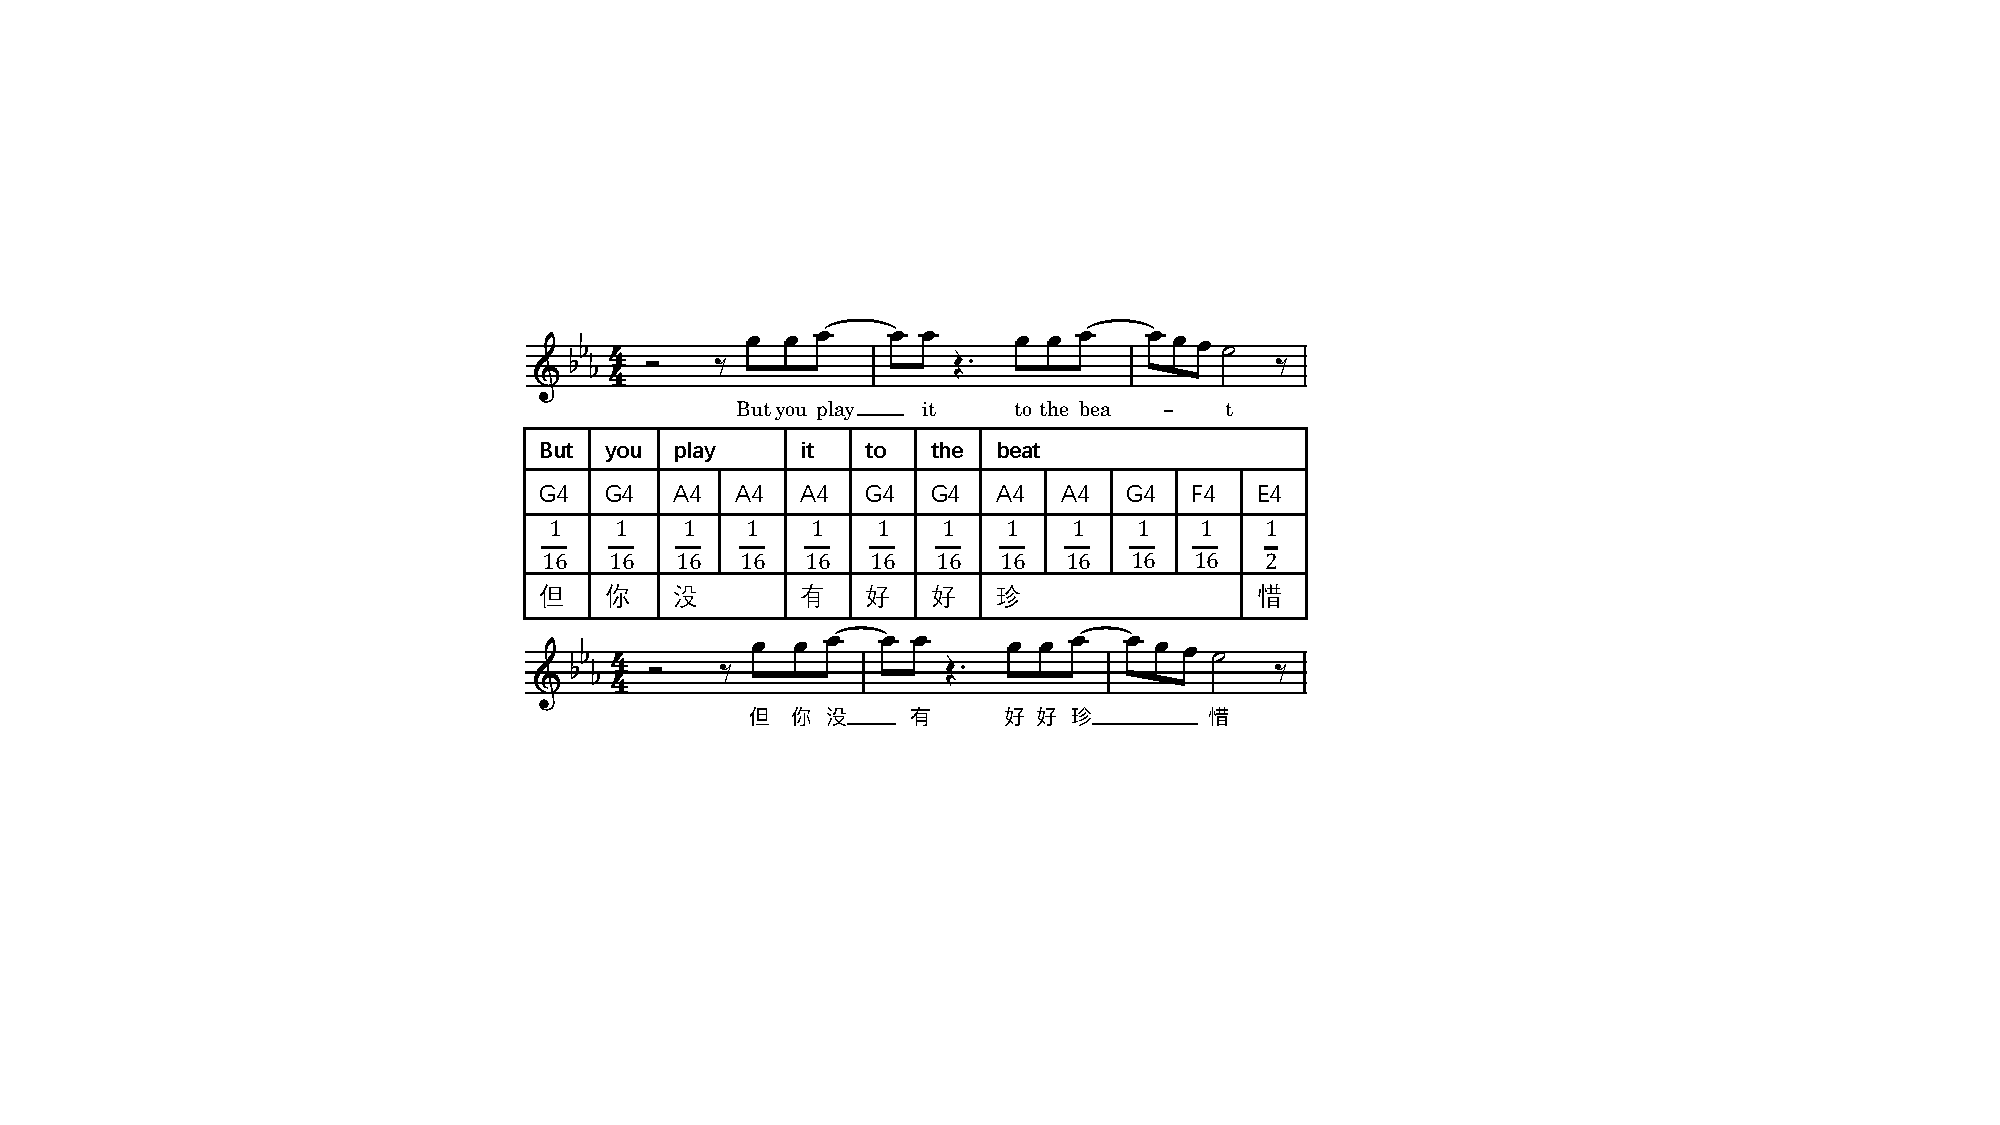
\includegraphics[width=0.99\textwidth]{figure/ast/exp.pdf}
  \caption{以\textit{Rolling In the Deep}一曲中``But you play it to the beat''一句的完整歌曲翻译为例。}
  \label{fig:task_exp}
\end{figure}
然而,尽管机器翻译(Machine Translation,MT)技术,尤其是神经机器翻译~\citep{nmt, vaswani2017attention, hassan2018achieving}(Neural Machine Translation,NMT)的进步,自动歌曲翻译在自然语言处理学界中并未得到充分的研究探索。这其中客观存在的一些挑战包括缺乏收集平行歌词和对齐数据的高效方式、难以对文本和旋律之间的复杂交互进行建模以及没有对乐谱规定的演唱方式进行直观评估的方式。歌曲翻译虽然与文本翻译密切相关,但本质上是一项更复杂的任务。除了在翻译中如用词和词序这样的考虑之外,歌曲的人工翻译者还需要具有目标语言的背景,能理解源语言并作出目标语言中诗意化的表达。此外,如图\ref{fig:task_exp}所示,翻译的歌词需要与旋律合理地对齐来保持歌曲的美感,这是歌曲翻译中不可缺少的要素~\citep{three_d_of_singability}。

此前,学界也探索过歌声合成 (Singing Voice Sythesis,SVS)这一技术来自动化地合成歌曲的人声演唱,并提出了一些在给定歌词和歌谱的情况下产生具有真实人声音色的、自然的、准确的歌声的方法。这样的方法不但使得对歌曲翻译结果方便而直观的评估成为可能,而且也为自动写歌谱曲、自动歌曲翻译这样的研究任务的实际落地奠定了基础。然而,自动歌曲翻译方向上的研究和歌声合成相比很少。作为目前为数不多的工作之一,~\citet{gagast}专注于通过在神经机器翻译的推理过程中施加特定约束来匹配有声调语言的翻译目标词语和旋律的音调、节奏等来得到更加合适、不易造成误解的翻译歌词。然而,\citet{gagast}直接使用文本翻译模型并对音符和字符之间对齐的严格规定一对一的匹配,无法捕捉到歌曲翻译更复杂的本质——即歌词和歌词-旋律对齐之间的关系。虽然音符的数量可以当作是翻译长度的一个简单上限,但正如\citet{interplay_lyrics_melody}一文中所观察到的现象,歌词和旋律之间的微妙对齐不应仅为简单而严格的规则所决定。


为了解决上述技术挑战,我们提出了带有自适应分组的歌词-旋律共同翻译模型,这是自动歌词翻译问题的第一个完整的技术解决方案,通过在基于Transformer的编码器-解码器框架内对歌词翻译和歌词-旋律对齐进行联合建模,我们提出的模型翻译出的歌曲既忠实于原歌词,又符合旋律,无论是客观指标还是主观评测都显示出模型翻译表现的优越性。
\section{章节安排}
本文各章节组织如下:


第一章:绪论。第一章节主要介绍了歌曲翻译技术和歌声合成技术的定义、应用和发展情况、自动歌曲翻译和歌声合成的国内外研究现状、以及自动歌曲翻译和歌声合成的研究背景及意义。另外,第一章节还阐述了本文将基于Transformer Encoder-Decoder模型和歌词和歌词-旋律对齐的关系来研究自动歌曲翻译任务、基于扩散模型来研究歌声合成任务,并探究xxx对于自动歌曲翻译和xxx对于歌声合成效果的影响。

第二章:相关研究介绍。

第三章:自动歌曲翻译研究

第四章:基于扩散模型的歌声合成研究。

第五章:歌曲到歌声翻译系统实践。

第六章:总结和展望。
\section{章节小结}

\chapter{相关研究综述}
本文的研究对象涉及自然语言处理的多个子领域,本章将分领域分别介绍歌曲歌词生成及限制性翻译和歌声合成相关技术的研究现状和近期进展。
歌曲歌词生成及限制性翻译目前有多个技术路线,分别着重于对自回归翻译的不同阶段施加限制,另外也有一些条件性歌词生成和对齐的相关技术与自动歌曲翻译这一任务相关。
歌声合成技术自语音合成发展而来,在语音合成方面,许多工作尝试以各类合成模型为基础搭建声学模型。这些模型因各自原理和结构不同,在模型规模、推理速度、训练难易度和合成表现上也各有千秋。
以下分别对这些子领域进行阐述。
\section{歌曲歌词生成及限制性翻译研究综述}
\label{sec:seq2seq}
歌词自动翻译研究历经基于规则的方法的阶段、统计机器翻译方法阶段和使用具有节奏和词汇句法约束的有限状态机阶段\citep{spanish_verse, Manurung2004AnEA, He_Zhou_Jiang_2012},近年来也逐渐开始引入神经网络模型向神经机器翻译靠拢
\citep{ghazvininejad-etal-2016-generating,ghazvininejad-etal-2017-hafez, ghazvininejad-etal-2018-neural}。
在语言学研究中,传统人工歌曲翻译研究通过利用语言学知识在歌词翻译和歌词旋律对齐方面都取得了一些进展
~\citep{interplay_lyrics_melody,low_2003,low2008translating,low_2022,three_d_of_singability,trans_of_music}.
当然,这些研究针对的对象都是专业歌手创作的歌曲,这些方法追求在一些有代表性的曲目中进行高质量的歌词翻译和歌词旋律对齐,力求达到``信、达、雅''的三重境界。
\begin{figure}[ht]
  \centering
  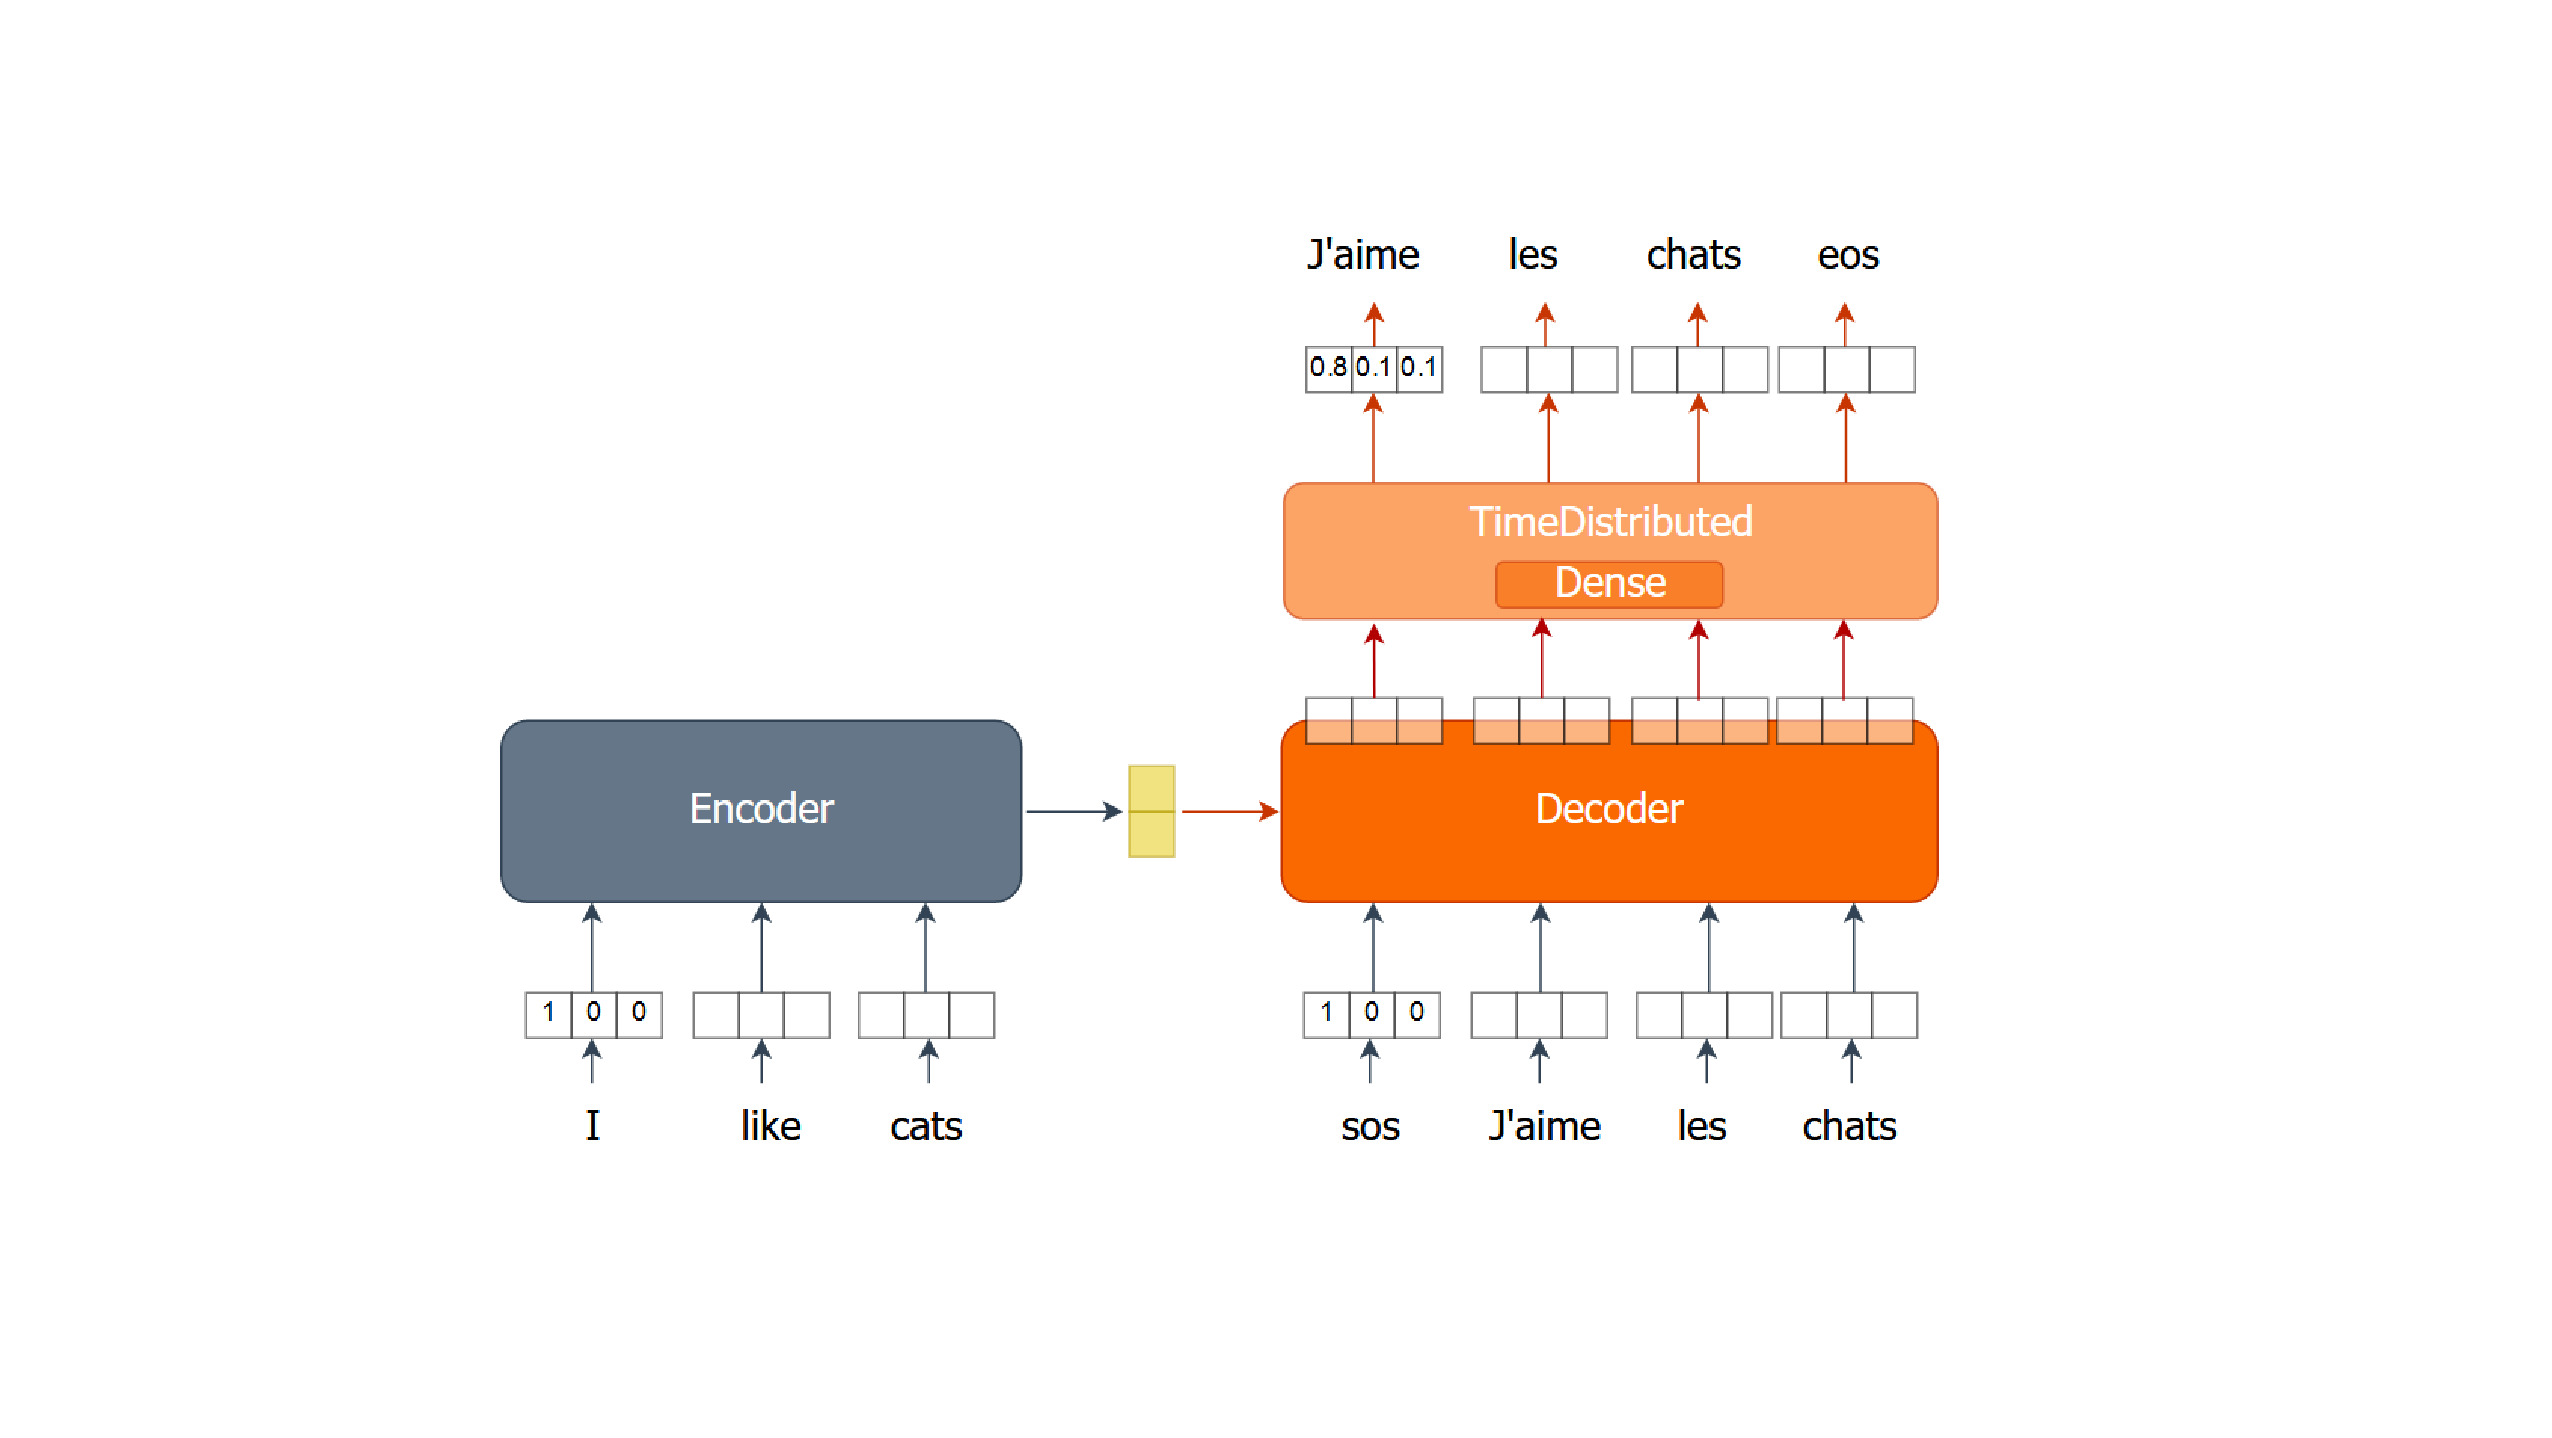
\includegraphics[width=0.99\textwidth]{figure/related/teacher-forcing.pdf}
  \caption{Teacher-forcing训练方式图示}
  \label{fig:tf_train}
\end{figure}
\subsection{基于序列生成的歌词生成、限制性生成和翻译研究}
% \subsubsection{限制性生成和翻译研究}
在近来基于神经机器翻译的工作\citep{gagast}中,自动歌曲翻译大多被当作一种存在一定限制条件的文本翻译任务进行建模。目前,文本翻译作为一种序列生成任务,大都采用自回归式的解码方式,而以Teacher-forcing方式进行训练以加快收敛。
基于此,很多工作~\citep{hokamp-liu-2017-lexically,zou_controllable,relyme}尝试仅在解码过程中直接对解码搜索时的评分施加目的性限制来进行重评分,让符合限制的结果得分更高,不符合的得分减少。如限制符合诗词格式、限制符合某些语法规则等。
解码时对结果的评分原本只有来自神经网络训练出的语言模型根据编码器的输入和已经解码出的前文对当前位置应解码结果的概率估计:
\begin{equation}
  P(y_t|y_0,y_1......y_{t-1}, X)
\end{equation}
现在则需要根据是否符合限制的判断进行重评分:
\begin{equation}
  P(y_t|y_0,y_1......y_{t-1}, X)+f(y_0,y_1......y_{t-1}, \mbox{restrictions})
\end{equation}
\begin{figure}[ht]
  \centering
  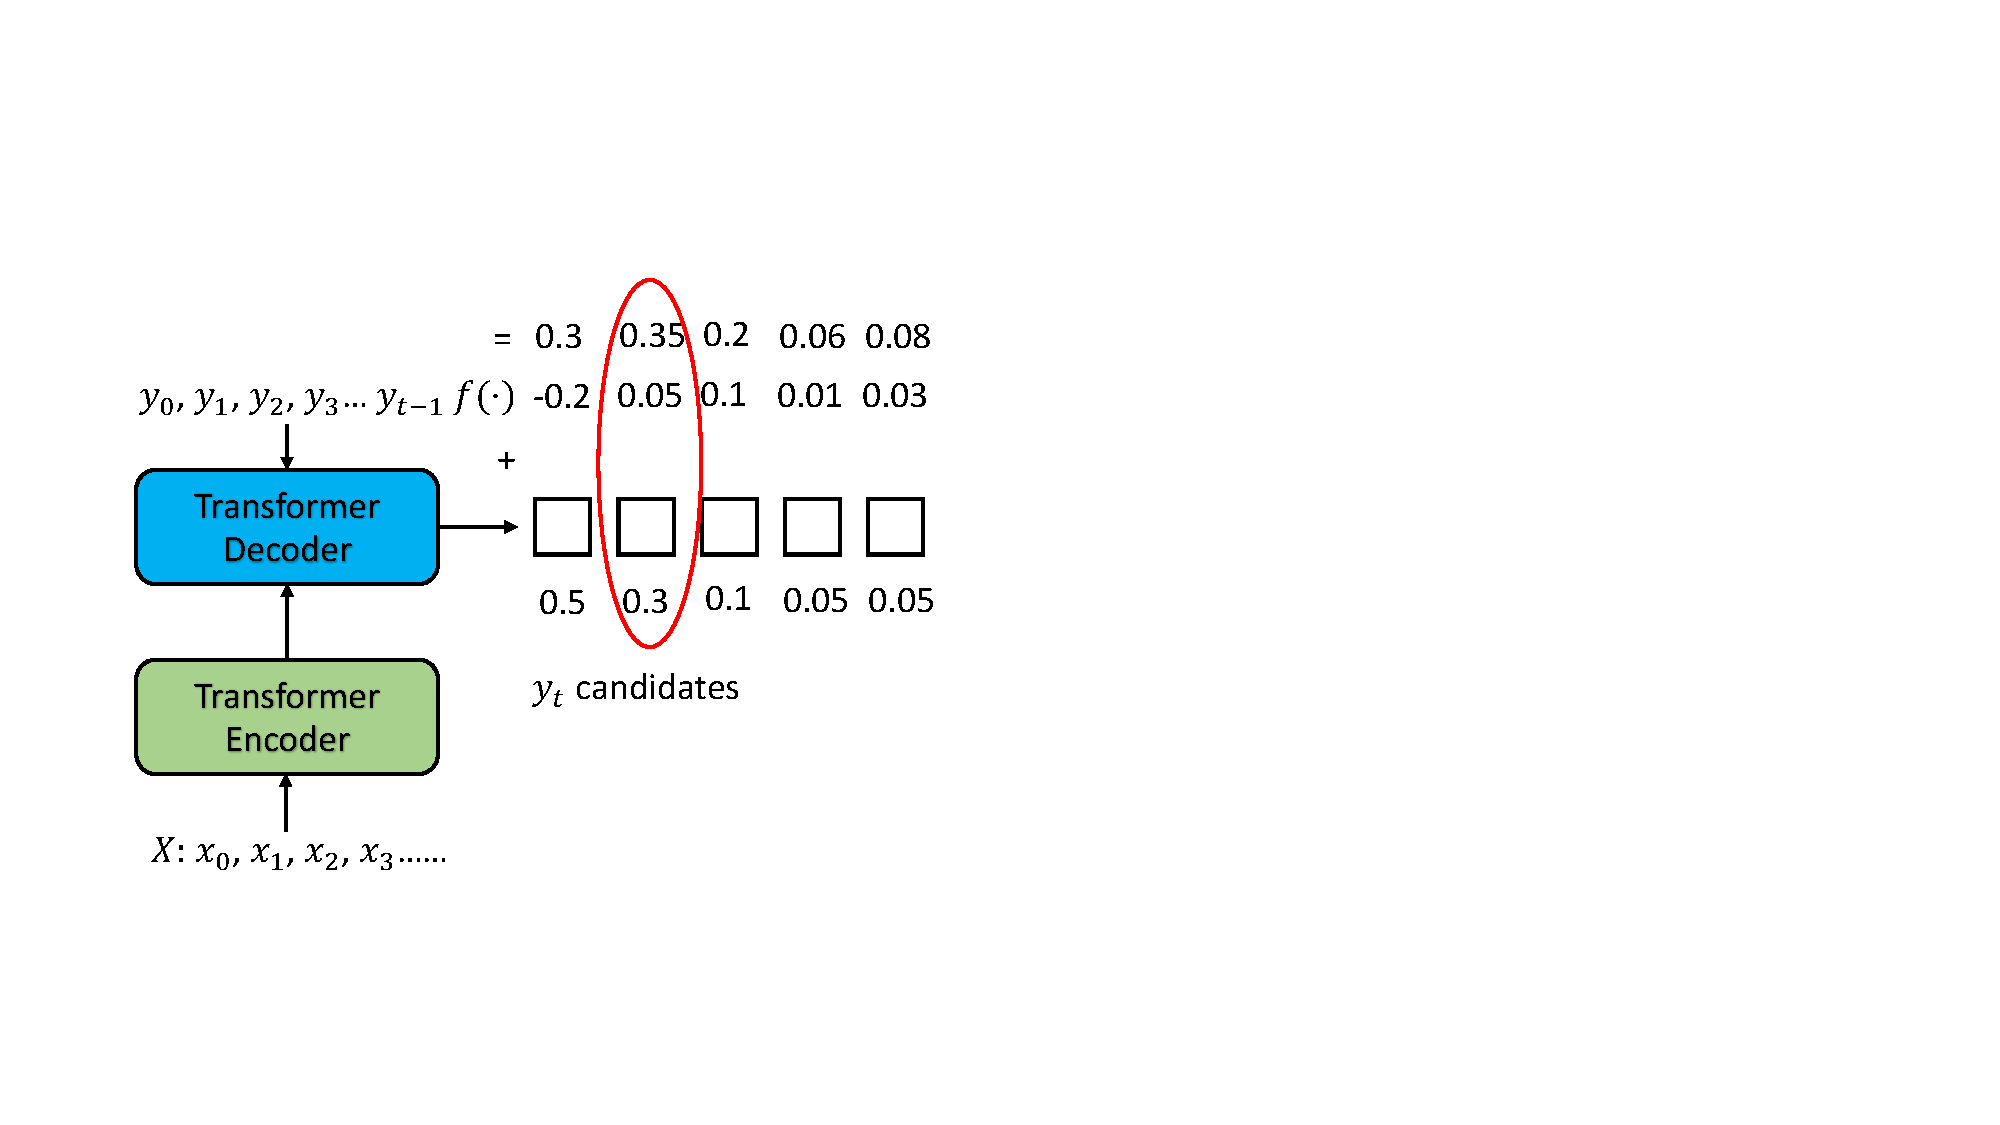
\includegraphics[width=0.80\textwidth]{figure/related/decoded_constrain.pdf}
  \caption{对解码搜索进行目的性限制的示例。}
\end{figure}
如\citet{relyme}一文中设计了代价函数来限制音调、轻重拍等以提升解码出的歌词和旋律的契合度:
\begin{equation*}
  R_r(y_{0:t-1},x) = \left\{
  \begin{array}{rcl}
    1, & & {\mbox{如果当前歌词符合节奏型要求}} \\
    0, & & {\mbox{不符合}}
  \end{array}
  \right.
\end{equation*}
% \citet{}中则将代价函数用于:
% \begin{eqnarray}
%
% \end{eqnarray}
此方面工作的探索证明了这类比较直接的做法大部分都比较有效,而且对于一些本质比较简单的限制来说,这种做法所需的编码工作量小,实施起来非常方便,而且无需对已经训练好的神经网络模型做其他调整。

除此之外,很多相关工作尝试在训练过程中施加约束,如在输入中添加与格式限制有关的嵌入表示作为条件,以在推理时通过输入的条件控制解码~\citep{li-etal-2020-rigid}或引入特殊词语以达到长度控制的目的~\citep{lakew-etal-2019-controlling,saboo-baumann-2019-integration}等。这些方法通过在输入时引入额外的条件作为控制信息,在训练时通过相应的结果监督来使得模型依赖控制信息对最终结果产生的影响,进而在推理时通过提供不同的控制信息来控制解码结果。这些数据驱动的方法同样表现出良好的性能,且能施加更加复杂的限制,模型表现更可靠。但是和仅干预解码过程的做法相比,限制的变动都需要设计和训练模型学习限制的方式。
\begin{figure}[!h]
  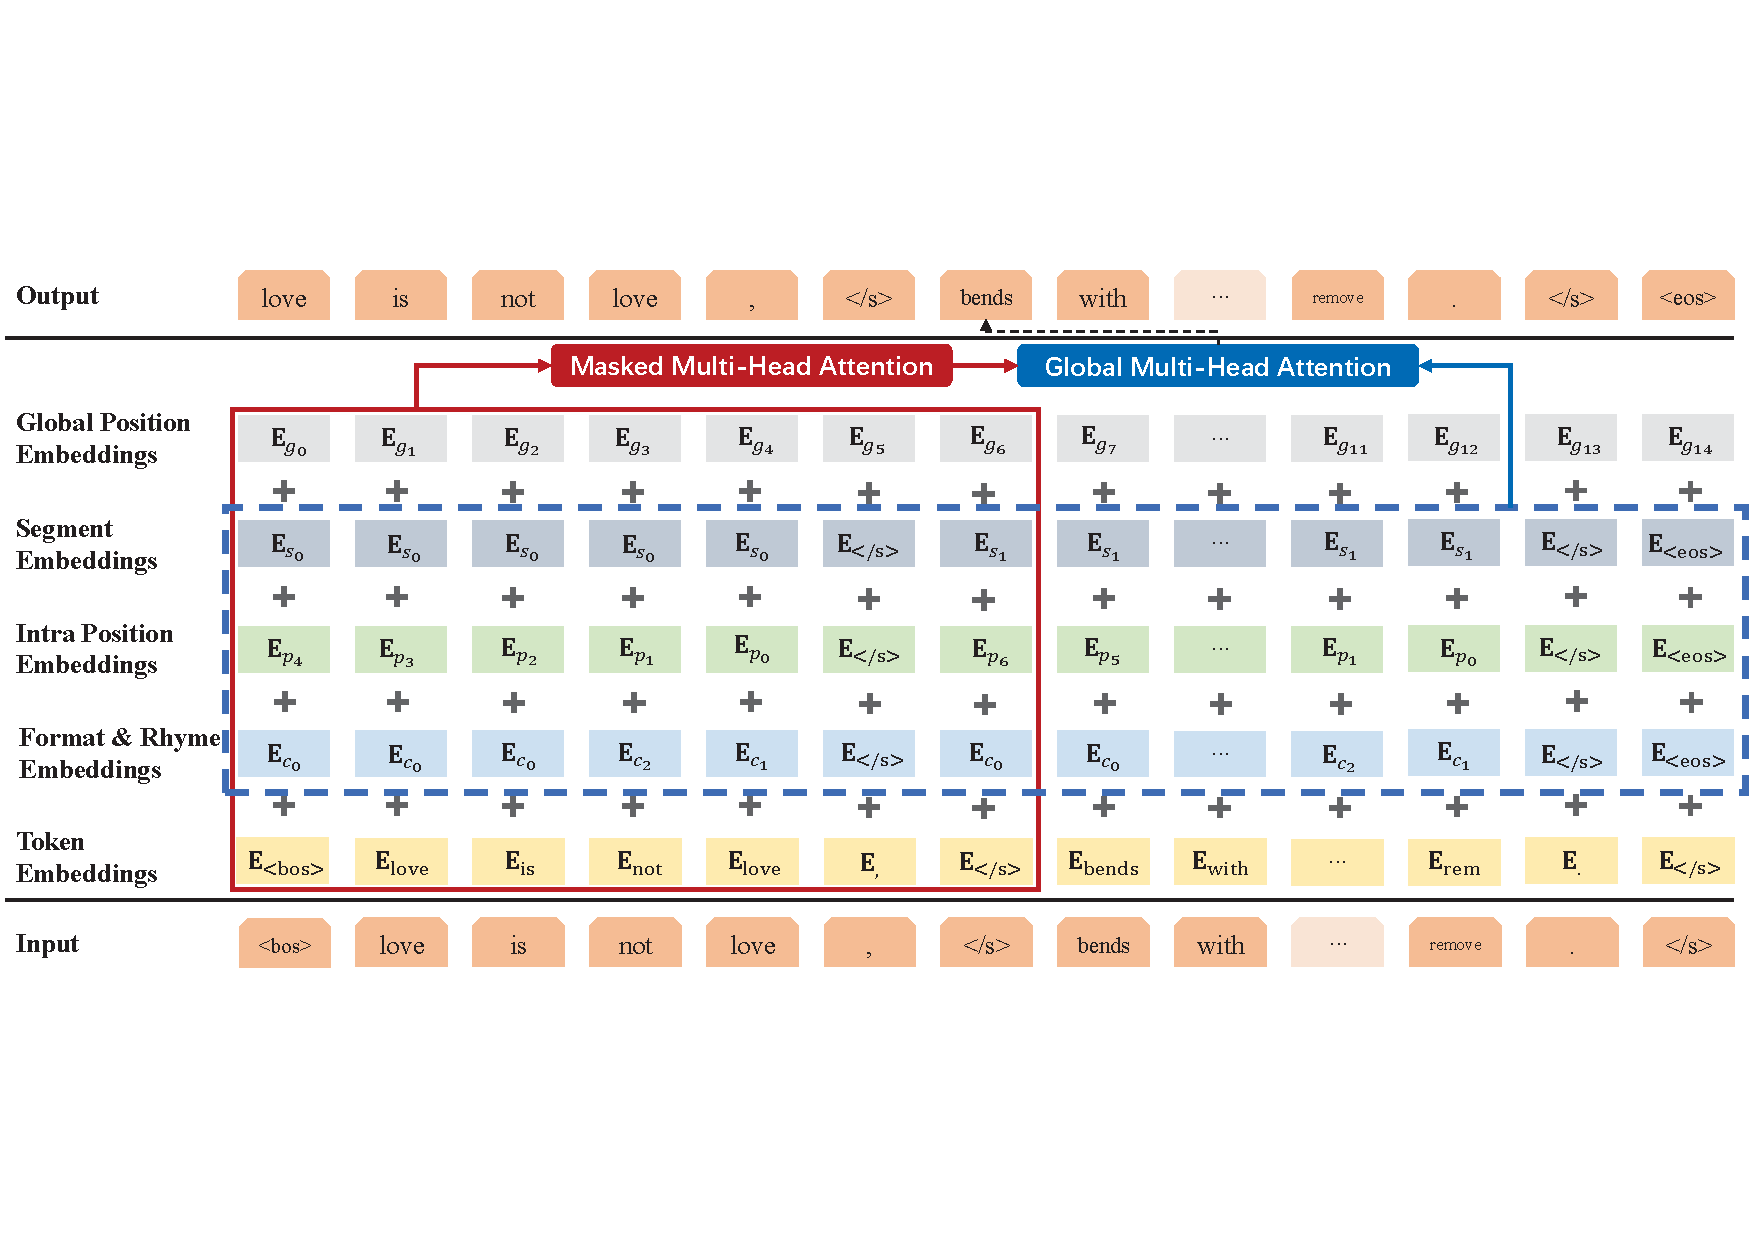
\includegraphics[width=0.99\textwidth]{figure/related/train_constrain.pdf}
  \caption{\citet{li-etal-2020-rigid}中在训练中限制生成的宋词诗句格式的模型示意图。}
\end{figure}
% \subsubsection{自动歌词生成研究}

在下一章中,本文将提出歌词旋律对齐和歌词共同翻译模型,在翻译的语料上进行翻译域偏移适应,同时也对翻译文本结果进行长度限制。
\subsection{歌词-旋律对齐预测方法}
\subsubsection{基于注意力机制的歌词-旋律对齐预测}
包含歌词旋律对齐预测的歌词生成是自动歌曲制作中最重要的任务之一,近年来随着神经网络模型在自动写歌谱曲任务中的进展。
近期的工作~\citep{lee-etal-2019-icomposer,Chen2020MelodyConditionedLG,songmass,telemelody,ai_lyricist,xue-etal-2021-deeprapper}绝大部分都使用了神经网络进行序列生成的模型框架,但是各自的侧重点不太一样。
有些工作关注如何限制生成结果的和节奏的对齐,也有写工作专注于限制了生成文本的主题或适配歌曲的类别。
一些工作~\citep{songmass,telemelody},如图\ref{fig:attn_diag},提出利用既定歌词和旋律间的注意力机制,
\begin{figure}[ht]
  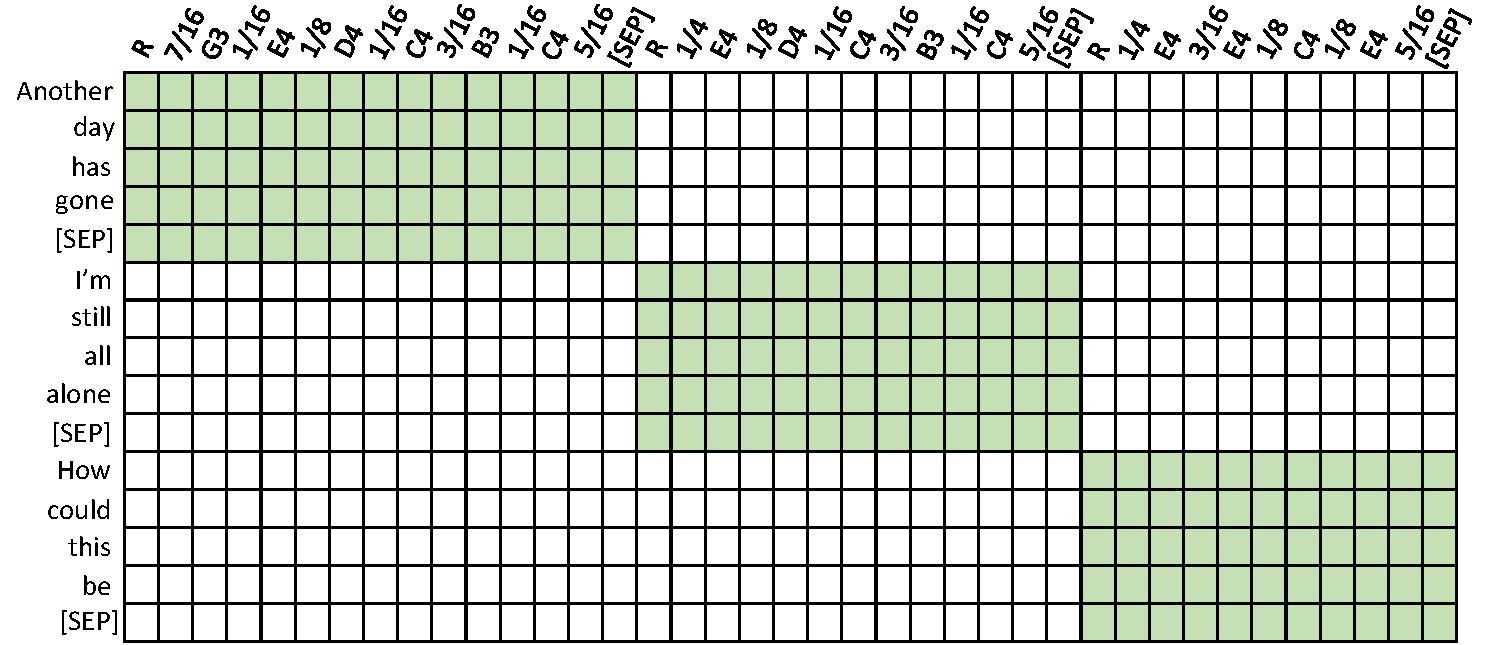
\includegraphics[width=0.99\textwidth]{figure/related/digattn.pdf}
  \caption{歌词和旋律之间的注意力权重矩阵示意图。}
  \label{fig:attn_diag}
\end{figure}
\begin{figure}[ht]
  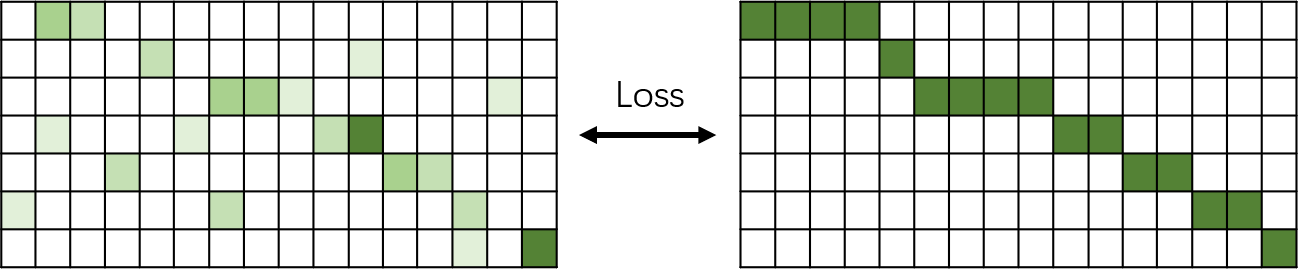
\includegraphics[width=0.99\textwidth]{figure/related/GuidedAttention.png}
  \caption{真实的对齐情况可以对歌词和旋律之间的注意力权重矩阵进行监督。}
  \label{fig:attn_loss}
\end{figure}
通过在注意力权重值的矩阵上进行动态规划算法求得最短路来找到歌词旋律之间合适的对齐方式。
% \begin{algorithm}[h]
% 	\caption{\label{alg:dp}求歌词-旋律对齐的动态规划算法\citep{songmass}}%算法标题
% 	\begin{algorithmic}[1]%一行一个标行号
% 	%    \STATE \textbf{Input}: Attention matrix $A \in \mathbb{R}^{(N+1) \times (M+1)}$. $N$, $M$ are the number of the tokens in source and target sentence. $A[0, :]$ and $A[:, 0]$ are set as zero first.
% 	    \STATE \textbf{Input}: 注意力权值矩阵$A \in \mathbb{R}^{N \times M}$,分数矩阵$F \in \mathbb{R}^{(N+1) \times (M+1)}$, 路径矩阵$\text{Path}$,源旋律序列$x$,目标歌词序列$y$。$N$和$M$分别是旋律序列$x$和歌词序列$y$的长度。
% 	    \STATE \textbf{Output}: 相对齐的歌词-音符对列表 $D$.
% 	    \STATE \textbf{Initialize}: F初始化为$-\infty$。 $\text{Path}$初始化为一个$(N+1) \times (M+1)$的空矩阵。
% 	    \STATE {$F[0][0] = 0$}
% 	    \FOR{$i=1$ to $T$}
% 	    \FOR{$j=1$ to $S$}
% 	    \FOR{$k=0$ to $j-1$}
% 	    \STATE $\text{score} = F[i-1][k] + \sum_{h=k+1}^{j}A[i][h]$
% 	    \IF{$\text{score} \ge F[i][j]$}
% 	    \STATE $F[i][j] = \text{score}$, $\text{Path}[i][j]=(i-1,k)$
% 	    \ENDIF
% 	    \ENDFOR
% 	    \FOR{$k=0$ to $i-1$}
% 	    \STATE $\text{score} = F[k][j-1] + \sum_{h=k+1}^{i} \frac{A[h][j]}{i-k}$
% 	    \IF{$\text{score} \ge F[i][j]$}
% 	    \STATE $F[i][j] = \text{score}$, $\text{Path}[i][j] = (k,j-1)$.
% 	    \ENDIF
% 	    \ENDFOR
% 	    \ENDFOR
% 	    \ENDFOR
% 	    \STATE $m,n = M,N$
% 	    \WHILE {$m \ne 0$ \AND $n \ne 0$}
% 	    \STATE $i, j = \text{Path}[m][n]$
% 	    \STATE \text{向}D\text{中添加($x_{[j+1:n]}$,$y_{[i+1:m]}$)对}
% 	    \STATE $m, n = i, j$
% 	    \ENDWHILE
% 	    \RETURN $D$
% 	\end{algorithmic}
% \end{algorithm}
注意力矩阵本身除了受到来自相应任务的损失函数的监督以外,也会受到真实对齐方式在特定行列的监督。
然而,由于这种方法得出的对齐路径来自于某种对齐距离矩阵,在未加限制的情况下有时会导致一音符对齐多字的非单调性输出,并且自注意力机制模块在训练中也需要相对大量的数据。但最重要的一点则是这种方法的对齐组件是在得到翻译结果后提供类似于基于规则的固定约束,而不是在训练期间和翻译一起动态地学习对齐的继承,即类似于后处理网络,而不是动态学习对齐从而限制歌词生成的模块。而且对于翻译任务来说,计算旋律和歌词之间的注意力权重矩阵会带来额外计算开销,且对齐情况无法在自回归过程中影响歌词的翻译。
\subsubsection{自适应计算时间}
本文在后文中使用的自适应分组的做法实际上是自适应计算时间算法的变种。自适应计算时间方法是\citet{act}一文在2016年提出的,用于控制循环神经网络模型中每一个时刻重复运算的次数的算法,即使用算法来控制循环神经网络在时序顺序上的每一个时间步状态时的计算网络的深度。
\begin{figure}[ht]
  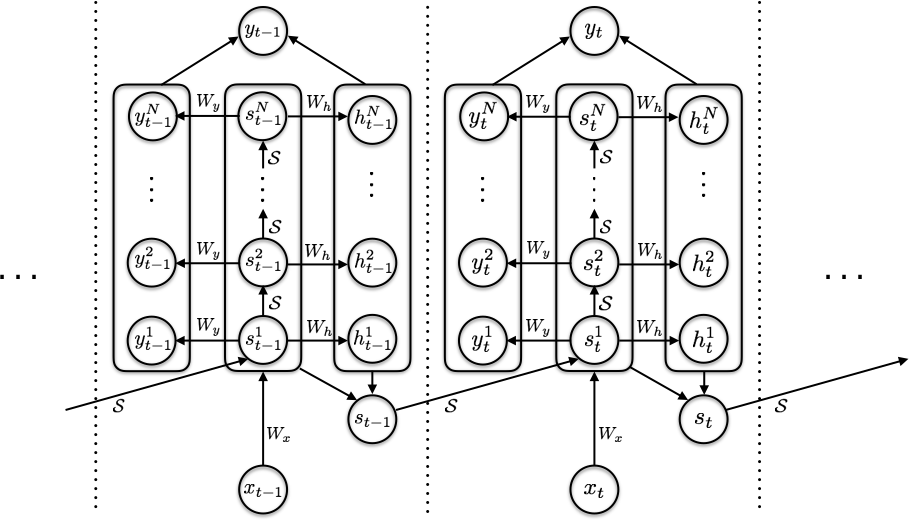
\includegraphics[width=0.99\textwidth]{figure/related/act.png}
  \caption{自适应计算时间控制循环神经网络的示意图。}
  \label{fig:act_rnn}
\end{figure}
如图\ref{fig:act_rnn}所示,自适应计算时间算法通过构建思考代价计算函数使得循环神经网络模型在时间步$t$时可以进行若干次迭代计算,迭代计算的思考代价会进行累加和作为时间序列在时刻$t$的输出。这种算法的核心逻辑为通过拉长循环神经网络在各个时间序列上的长度来增强模型的复杂性,提高模型的非线性表达能力。模型的损失函数为包含思考代价和任务目标的复合损失函数,所以自适应计算时间算法被设计为既鼓励神经网络快速进行判断而不是一味的追求精度消耗大量计算资源,又在一定代价内可以对循环步数进行延展提升网络复杂性。
\begin{equation*}
  \tilde{L}(x,y)=L(x,y)+\tau \sum_{t=0} P(x,t)
\end{equation*}
后续也有一些工作拓展了自适应计算时间方法,将其应用在Transformer等结构上来优化模型的计算。
本文提出的模型框架则是利用了歌词旋律对齐排列的单调性,进而通过自适应的分组算法设计了一个用于与翻译过程并行的进行对齐预测的轻量的神经网络。
\section{语音合成声学模型和扩散模型相关研究综述}
\subsection{语音合成和歌声合成声学模型相关研究介绍}
\label{sec:svs_intro}
语音合成研究起步于使用连接式的方法~\citep{macon1997concatenation,kenmochi2007vocaloid}或基于隐马尔可夫过程的参数化~\citep{saino2006hmm,oura2010recent}方法来合成目标音频。这两类方法在现在看来,流程都相对繁琐,且在内容和韵律上缺乏灵活性,音频听起来也不够和谐。由于深度学习的快速发展,在过去几年中,已经有多种基于深度神经网络的歌声合成系统被提出。\citet{nishimura2016singing,blaauw2017neural,kim2018korean,nakamura2019singing,gu2020bytesing}等工作率先尝试使用神经网络将语音内容的上下文特征映射为声学参数特征,进而合成线性频谱、梅尔频谱或功率谱等声学特征,或直接合成波形。
这些基于深度神经网络的合成方法大致可以分成自回归和非自回归两类,下面将分别进行阐述。
\subsubsection{时序自回归式的声学模型}
自回归类模型被提出的较早,其利用序列建模的方法,使用LSTM等循环神经网络对声音信号的线性频谱或梅尔频谱进行时序建模,一帧一帧地预测频谱的高低频情况。这一类模型的代表作就是Tacotron系列。
\begin{figure}[ht]
\centering
  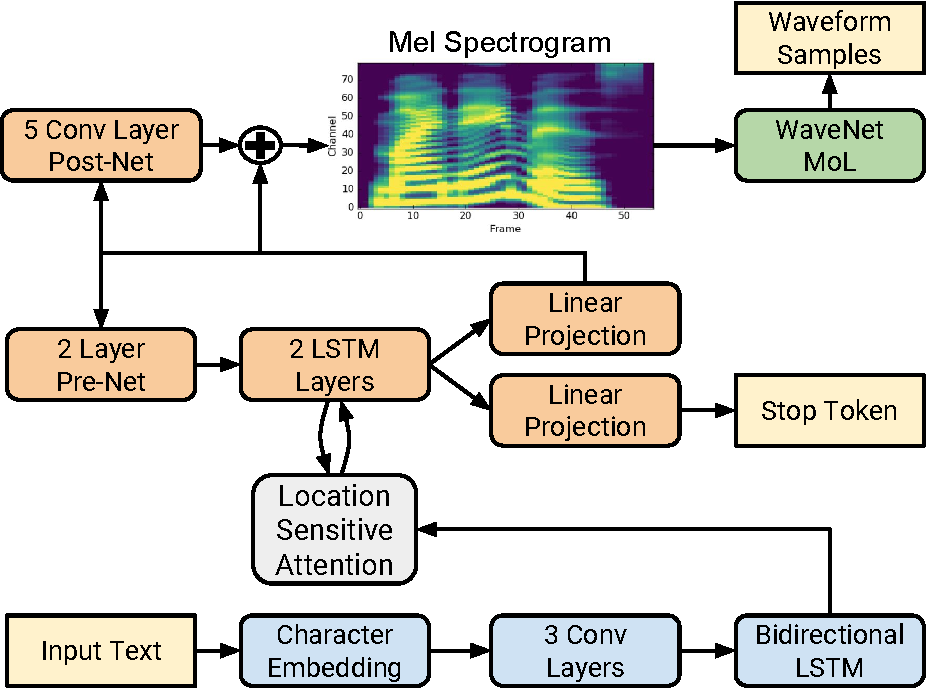
\includegraphics[width=0.80\textwidth]{figure/related/tacotron2.pdf}
  \caption{Tacotron声学模型示意图}
\end{figure}
Tacotron\citep{tacotron}构建的基于注意力机制的编码器-解码器框架将字符作为输入并输出线性频谱,使用Griffin-Lim算法\citep{GriffinLim}生成波形。Tacotron 2\citep{shen2018natural}则开始生成后续工作普遍采用的梅尔频谱并使用WaveNet\citep{vanwavenet}模型作为声码器并将梅尔频谱转换为波形。Tacotron 2和早期的连接式、参数式方法相比,合成的语音质量已经有了很大的提高。
后来也有许多工作尝试从不同方面改进和发展Tacotron系列。比如\citet{gsttacotron}、\citet{reftacotron}等在Tacotron原有框架基础上引入音频参考编码器和样式词来增强语音合成的表达能力。
\citet{nonattentivetacotron}和\citet{durian}则尝试替换Tacotron中的注意力机制,而使用一个单独的持续时间预测器进行自回归预测。
也有基于Tacotron构建端到端的文本直接生成波形的模型,如Wave Tacotron\citep{wavetacotron}。
基于Transformer结构的模型的提出最直接的动机就是使用循环神经网络构建的自回归模型有无法同时平行地训练和推理带来的模型效率问题和长频谱下自回归模型建模能力衰减的问题。
\citet{transformertts}提出使用基于Transformer的编码器-解码器的基本模型结构来从输入的音素直接生成梅尔频谱。
\citet{transformertts}除了Transformer结构以外,仍沿用了Tacotron 2的一些设计,达到了和Tacotron 2的相似质量的音质,但训练和推理速度更快。然而,与基于循环神经网络Tacotron系列模型相比,Transformer中的编码器-解码器的注意力计算不够稳定和鲁棒,因此,一些工作开始致力于增强基于Transformer的声学模型的鲁棒性,如对注意力矩阵添加对角化限制\citep{robutrans}等。
但由于自回归本身的训练会带来暴露偏差(exposed bias)问题,这种建模方法有一定的缺陷,在实际应用中反映出的问题就是拖音、漏音、静音过长、韵律预测不稳等现象。
\begin{figure}[ht]
  \subfloat[]{
    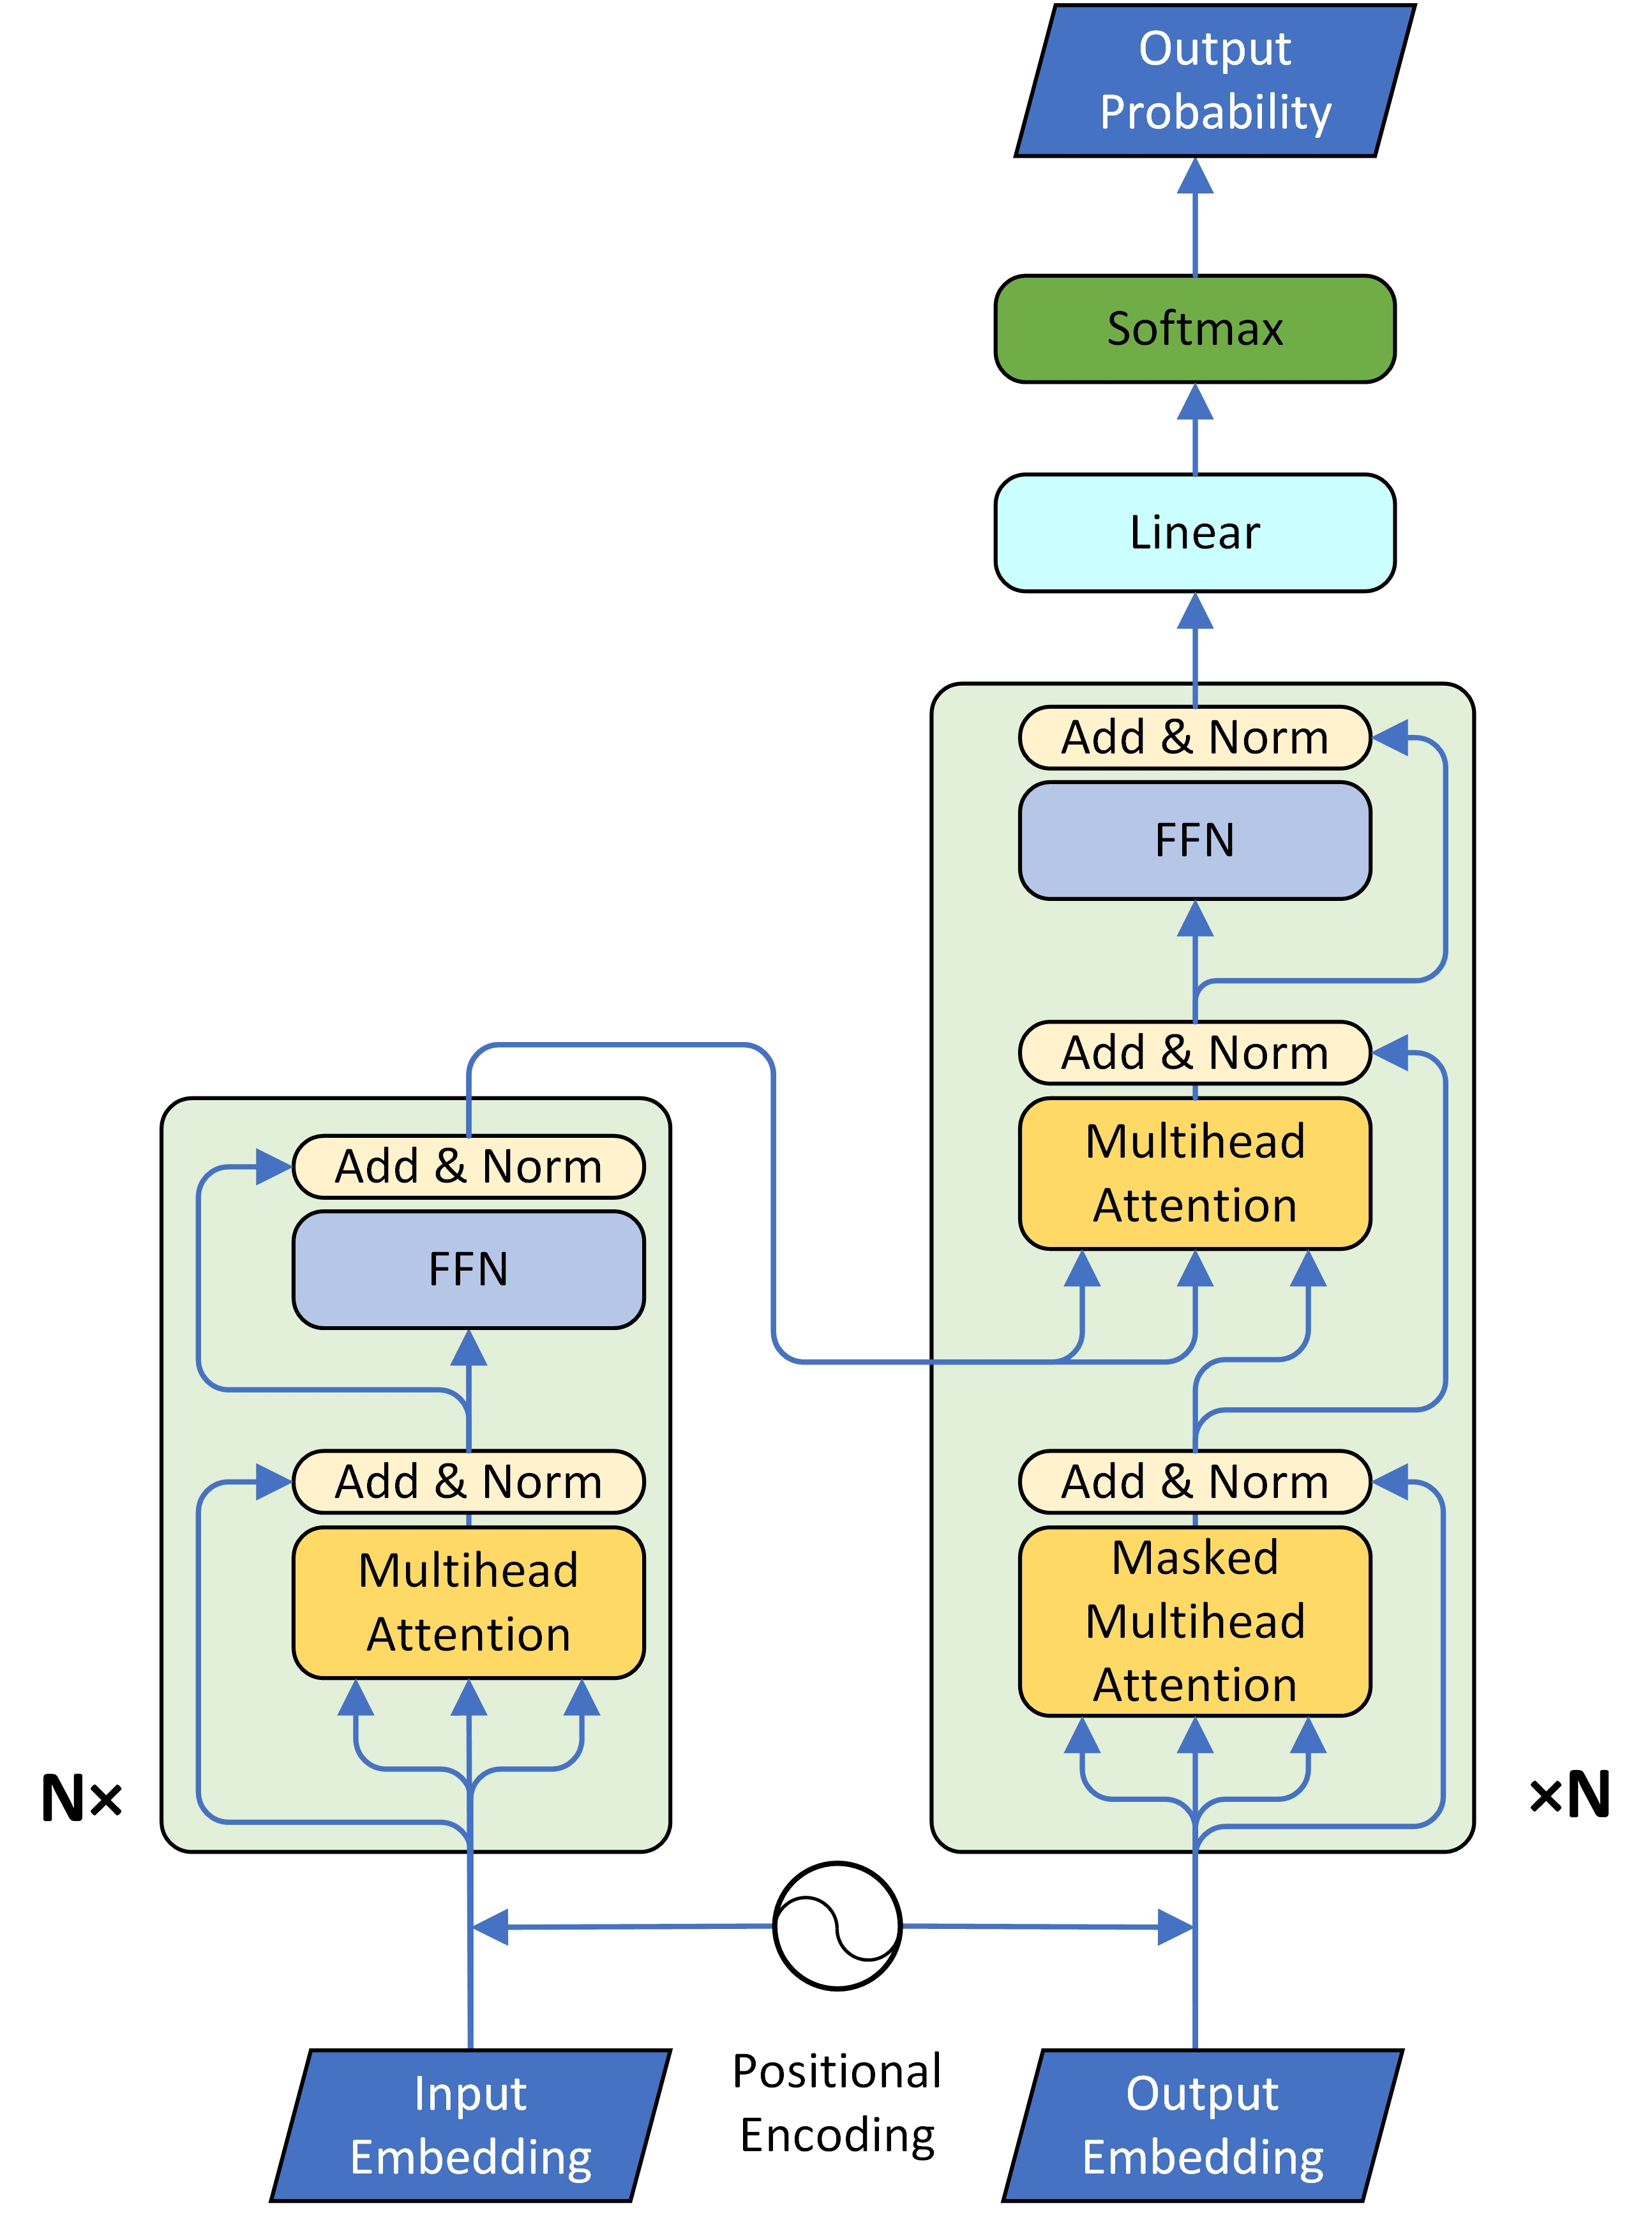
\includegraphics[width=0.49\textwidth]{figure/related/transformertts_a.jpg}
  }
  \subfloat[]{
    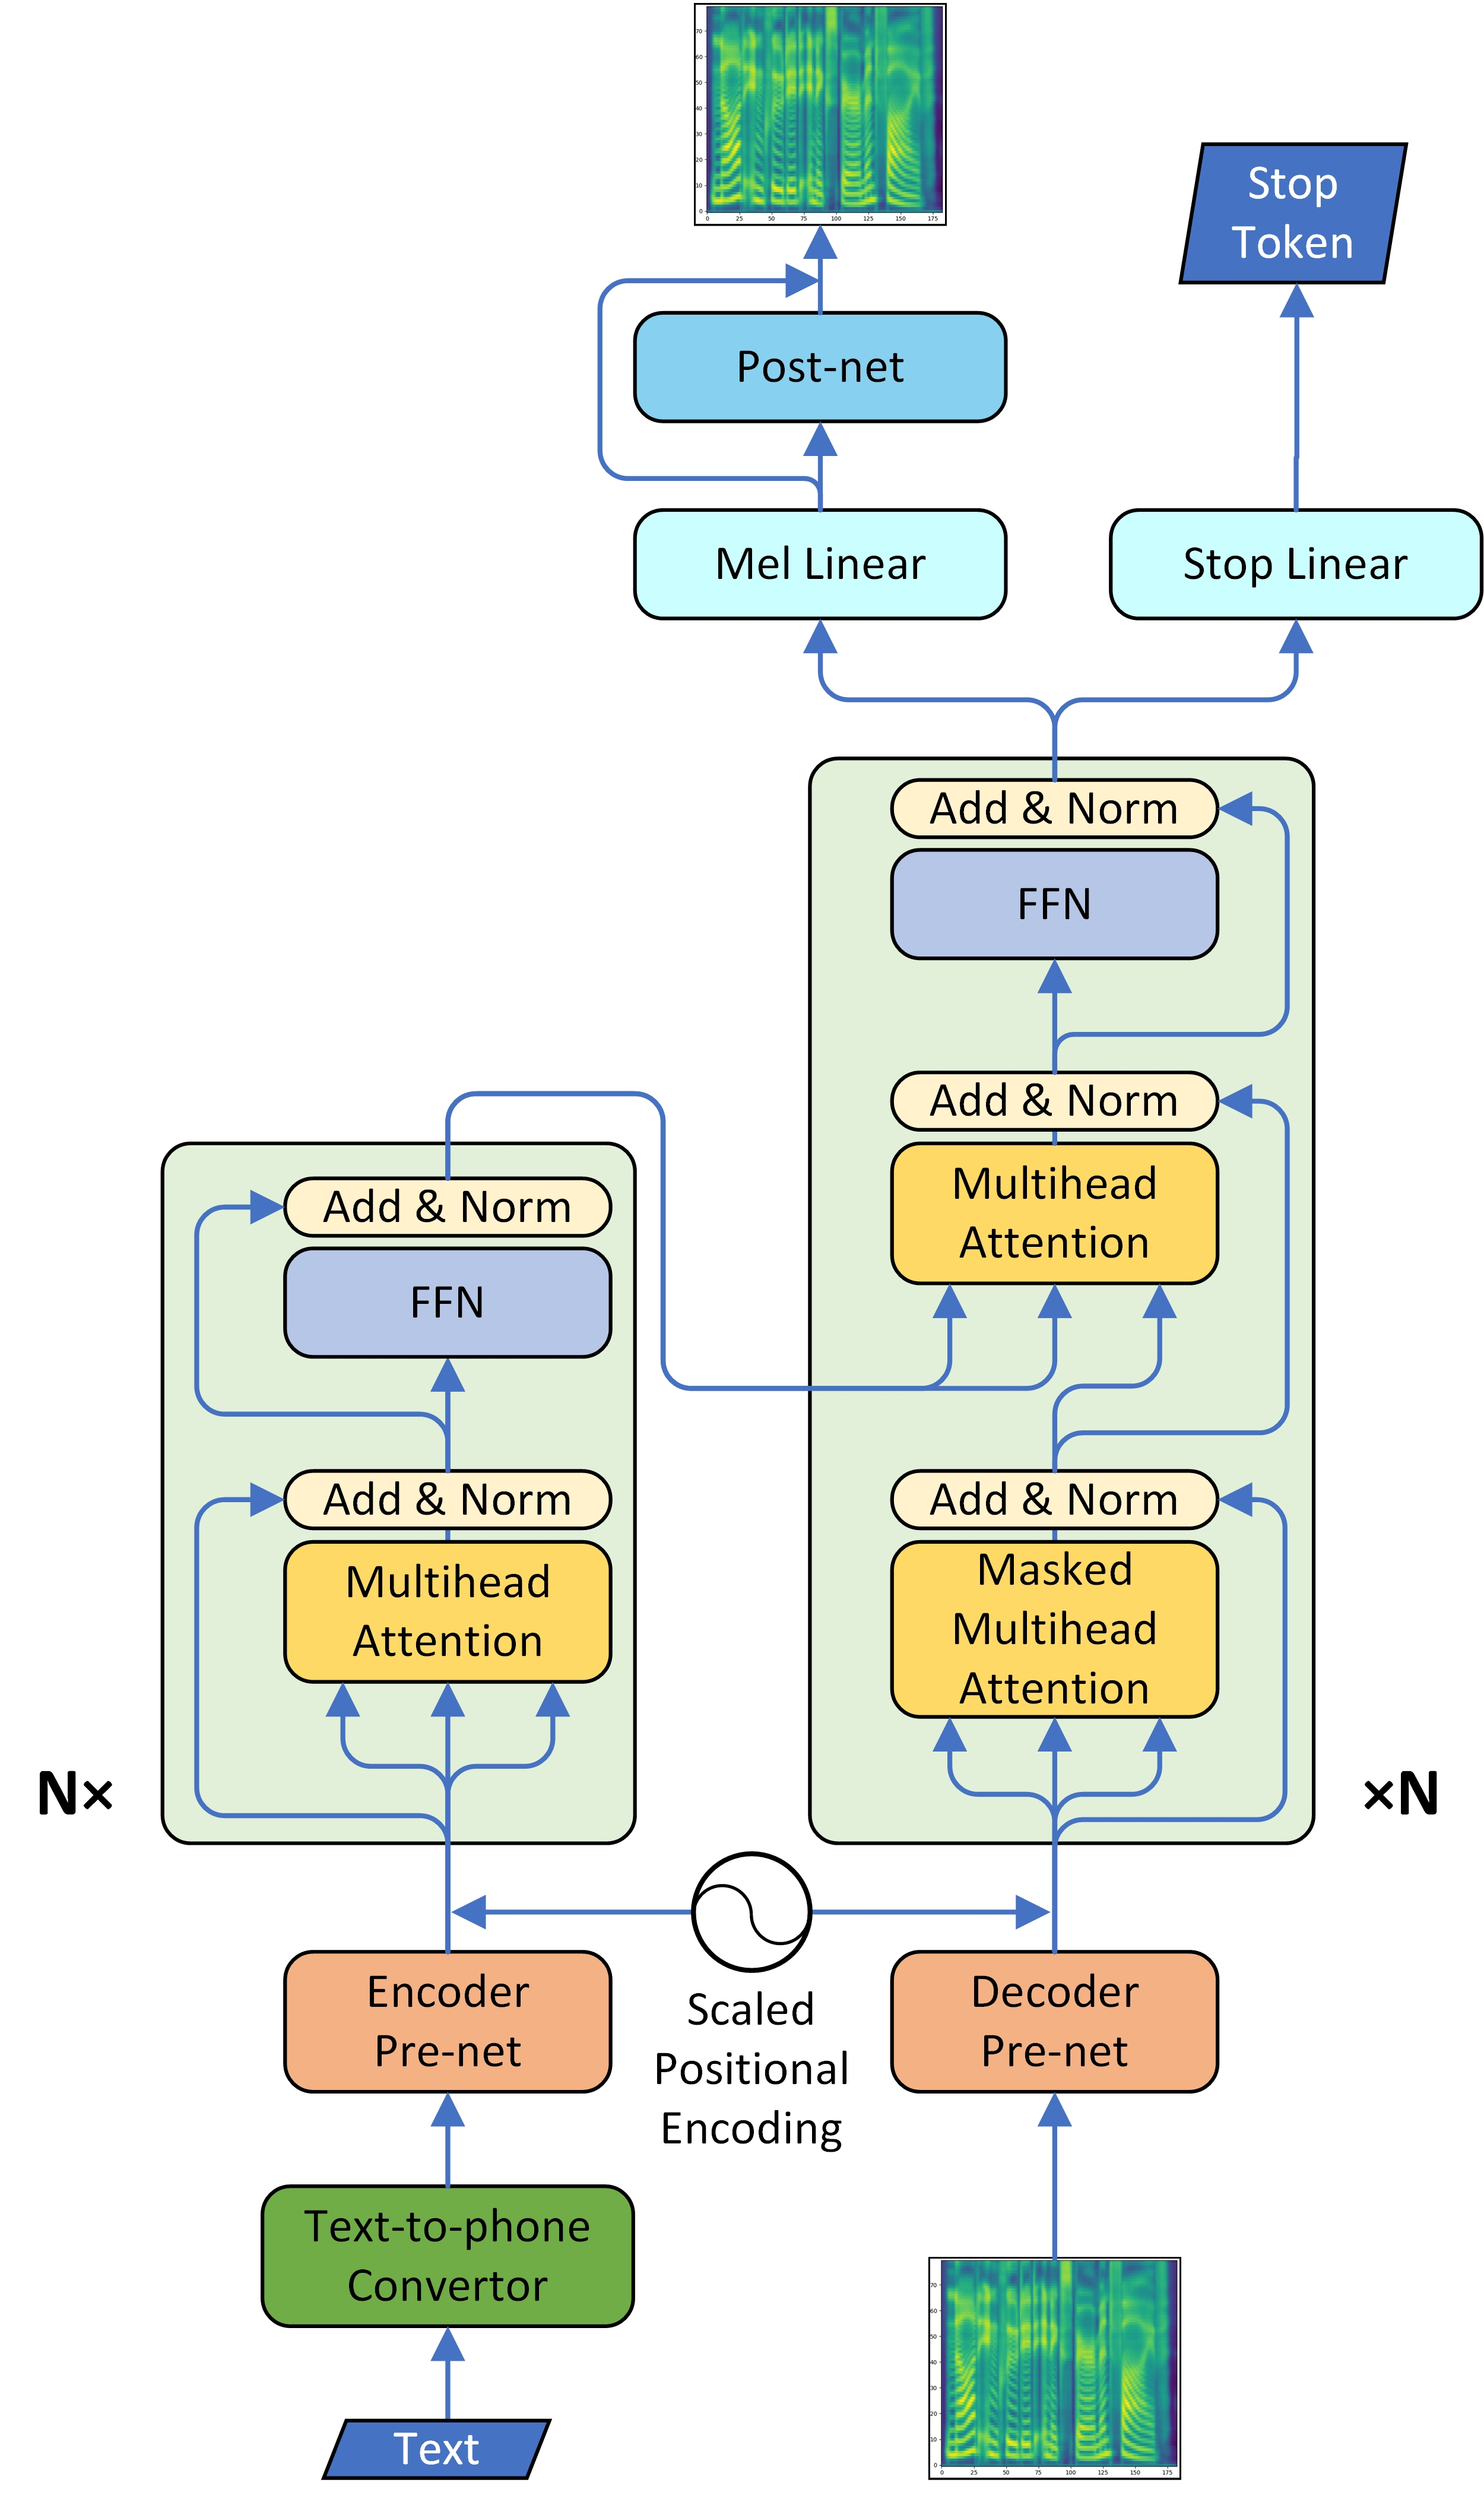
\includegraphics[width=0.49\textwidth]{figure/related/transformertts_b.jpg}
  }
  \caption{基于Transformer的自回归声学模型示意图}
\end{figure}
\subsubsection{非自回归式的声学模型}
非自回归类模型的提出相对较晚,但相关工作近年来层出不穷,从基于Transformer结构的模型到基于各类生成模型的结构,非自回归类的声学模型有后来居上的趋势。
无论是Tacotron系列,还是基于Transformer的自回归模型,都存在上节提到的两个问题:推理速度慢和鲁棒性问题。
自回归的梅尔频谱生成速度较慢,特别是对于较长语音序列有较多的语音帧需要生成时,因为推理时间开销与帧数是呈线性关系的。生成的语音也存在一定的漏音、重复等造成音频听起来很不自然的问题,这主要是由基于Transformer的编码器-解码器的自回归生成中,文本和梅尔频谱之间的注意力对齐不准确造成监督不准确引起的。
因此\citet{ren2019fastspeech}采用了基于前馈Transformer的模型来并行地生成梅尔频谱,同时,使用长度调节器来调节音素和梅尔频谱帧序列之间的长度关系,取代了文本和语音之间的注意力机制,以避免跳词和重复问题,因而提高了模型预测时的鲁棒性。
长度调节器是一个音素的持续时间预测器,用于预测每个音素的持续时间,模型根据音素持续时间来扩展音素的隐藏层表示序列,其中扩展的音素隐藏层序列可以匹配音素谱图序列的长度,就可以进行并行生成了。
\begin{figure}[htbp]
  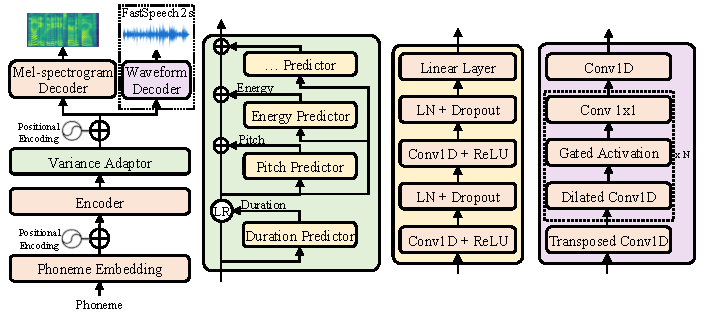
\includegraphics[width=0.99\textwidth]{figure/related/fs2.pdf}
  \caption{FastSpeech\citep{ren2019fastspeech}基于Transformer的非自回归声学模型示意图}
\end{figure}
从上述模型可以看出,非自回归类的模型由于需要在生成过程进行前先设定好长度,所以总帧数及基于各种语音特征的长度预测非常关键。一般的非自回归模型也可以通过已经训练好的自回归模型来引导时长预测训练或者引导特征的学习。

变分自编码器是一类通过引入隐变量分布并优化联合分布的变分下界而学习将常见分布变换为要建模的数据分布的生成模型,其构造的隐变量$z$通常来自连续分布,且各个维度可以进行解耦以对应语音中的人声特征、韵律特征和情感特征等,有利于降低解码器的重建难度,
\begin{figure}[!ht]
  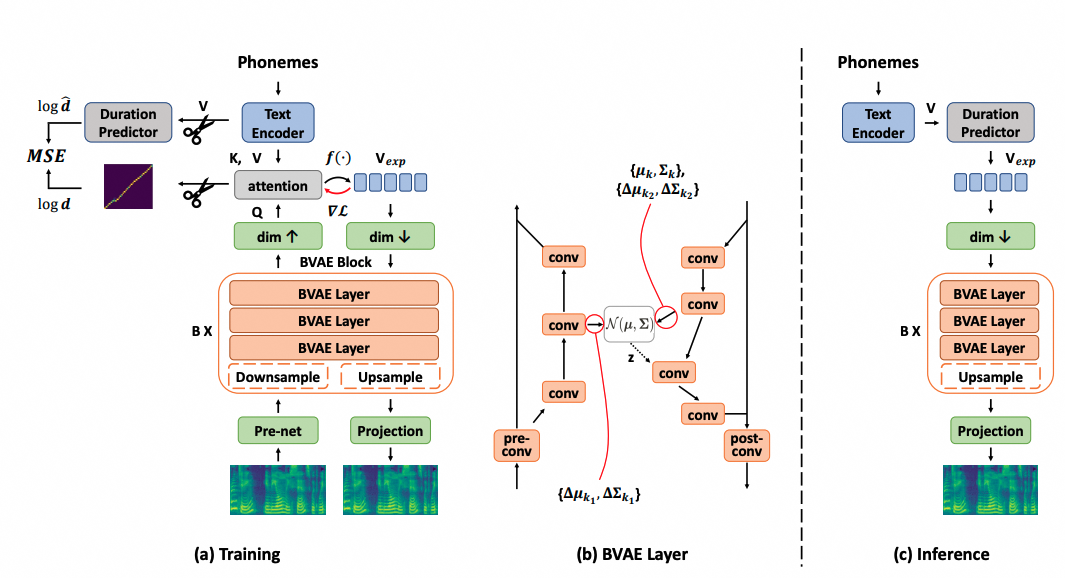
\includegraphics[width=0.99\textwidth]{figure/related/bvaetts.png}
  \caption{基于变分自编码器的声学模型示意图\citep{lee2020bidirectional}。}
\end{figure}

与变分自编码器类似,生成流模型也试图将输入分布编码为隐变量分布,但要求使用的变换可逆,所以其使用的网络结构相对受限,但通常网络整体更加轻量。
\citet{waveglow}和\citet{kim2020glow}提出了基于流模型的声学模型和声码器模型,其中\citet{kim2020glow}特别针对流模型的网络可逆特点,设计了单调对齐搜索算法来搜索最优的文本特征与流模型网络经过逆变换得到的语音特征的对齐信息,而后并行地生成最终的语音特征。
\citet{kim2020glow}一文提出的声学模型将音素、音调等条件信息合并到了生成流的概率分布的参数中,梅尔频谱通过基于生成流的解码器网络生成隐变量,文本序列通过编码器网络生成流的隐变量服从的高斯分布的均值和标准差,这样,两类特征就能寻找相应的映射矩阵并计算似然概率了。
\begin{figure}[htbp]
  \subfloat{
    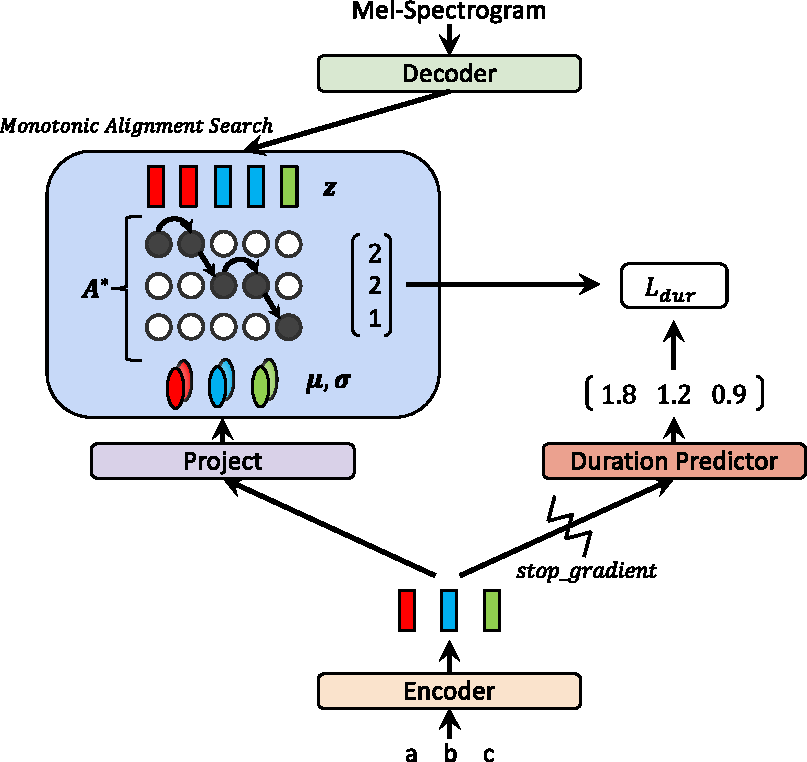
\includegraphics[width=0.49\textwidth]{figure/related/glowtts_a.pdf}
  }
  \subfloat{
    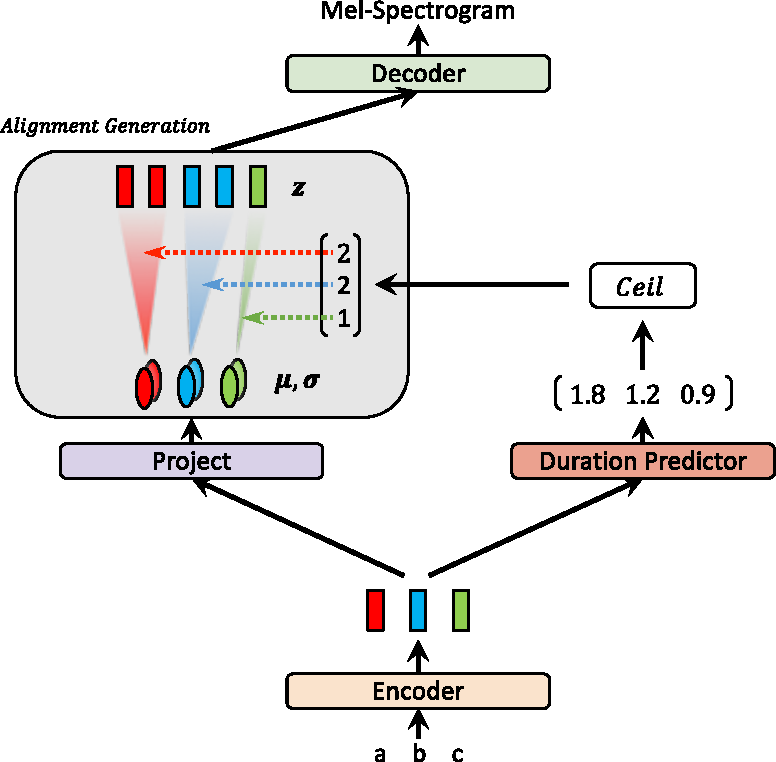
\includegraphics[width=0.49\textwidth]{figure/related/glowtts_b.pdf}
  }
  \caption{基于生成式流模型搭建的声学模型示意图}
\end{figure}
基于变分自编码器和生成流的声学模型,虽然推理速度快,对谐波轮廓的建模好,但是生成的频谱细节不佳,有模糊现象,对于音质特点和音频细节有一定伤害。由于歌声的表现力更加依赖人声的特殊音质特点和音频细节,上述缺陷在歌声合成中体现的更加明显。
% \subsection{歌声合成模型}

歌唱合成和语音合成相比起步较晚,其在语音合成任务受到学界关注时却未有类似热度的原因之一就是训练数据问题。歌唱合成的训练语料与普通语音相比,需要歌手在专业的录音棚录制的干声,且歌声的标注更为复杂,因而收集难度大,成本昂贵。
\citet{ren2020deepsinger}成功地使用了从音乐网站挖掘的歌唱数据从零开始构建了歌声合成系统,也为后续工作提供了一个方便可行的较低成本流程框架。\citet{blaauw2020sequence}则提出了一种基于前馈Transformer的非自回归歌声合成模型,推断过程快速,且能避免自回归模型引起的暴露偏差问题。
此外,对抗训练也是生成模型中的常用技术,最早由\citet{GAN}一文在2014年提出。其基本思想是将整体网络结构分为生成模型(Generator)和判别模型(Discriminator),其中
生成模型负责生成更接近真实分布的数据,让判别模型无以分辨,而判别模型则负责分类出真实数据和生成的数据。这两个模型协同交替,迭代地进行更新训练,通过二者之间的对抗训练模式使生成模型可以不断得到强化,获得更强的生成能力。最终生成模型就可以生成更接近真实样本的数据。
在对抗训练的帮助下,\citet{lee2019adversarially}~提出了一个直接生成线性频谱的端到端框架。\citet{wu2020adversarially}~则提出了一个可以利用数量有限的录音数据就能构建起来的支持多歌手的歌声合成系统,并通过使用多随机窗口鉴别器来提高合成语音质量。\citet{chen2020hifisinger}~在模型中引入了多尺度对抗训练,以相对较高的采样率(48kHz)合成高清音频。
不过虽然对抗训练对提升歌声合成模型的合成能力很有作用,但其本身存在这训练调参过程繁琐、生成模型和判别模型训练更新不稳定、难以收敛等问题。
% \begin{figure}[htbp]
%   \includegraphics[width=0.99\textwidth]{figure/related/gantts.pdf}
%   \caption{基于对抗训练的歌声合成模型示意图。\citep{}}
% \end{figure}
近年来,歌声合成系统的音频结果的语音自然度和多样性都在不断提高,已显现在24kHz和48kHz下媲美人声的潜力。
\subsection{扩散模型相关研究介绍}
扩散概率模型也一种是通过优化似然函数整体变分下界进行训练的参数化的马尔可夫链,这样一个参数化的随机过程能以恒定的时间步长生成与数据分布匹配的样本~\citep{Ho2020ddpm},其最大的优势在于整个过程对似然函数的计算更加精确,因而在理论上可以获得更好的数据分布拟合效果。
扩散模型首先由\citet{sohl2015deep}一文在2015年提出,之后的工作\citet{Ho2020ddpm}~又对最初的扩散模型进行了改进,以使用特定的参数化方式生成高质量图像,也揭示了扩散模型与去噪梯度得分匹配之间的等价性~\citep{song2019generative,song2021scorebased}。
\begin{figure}[!h]
  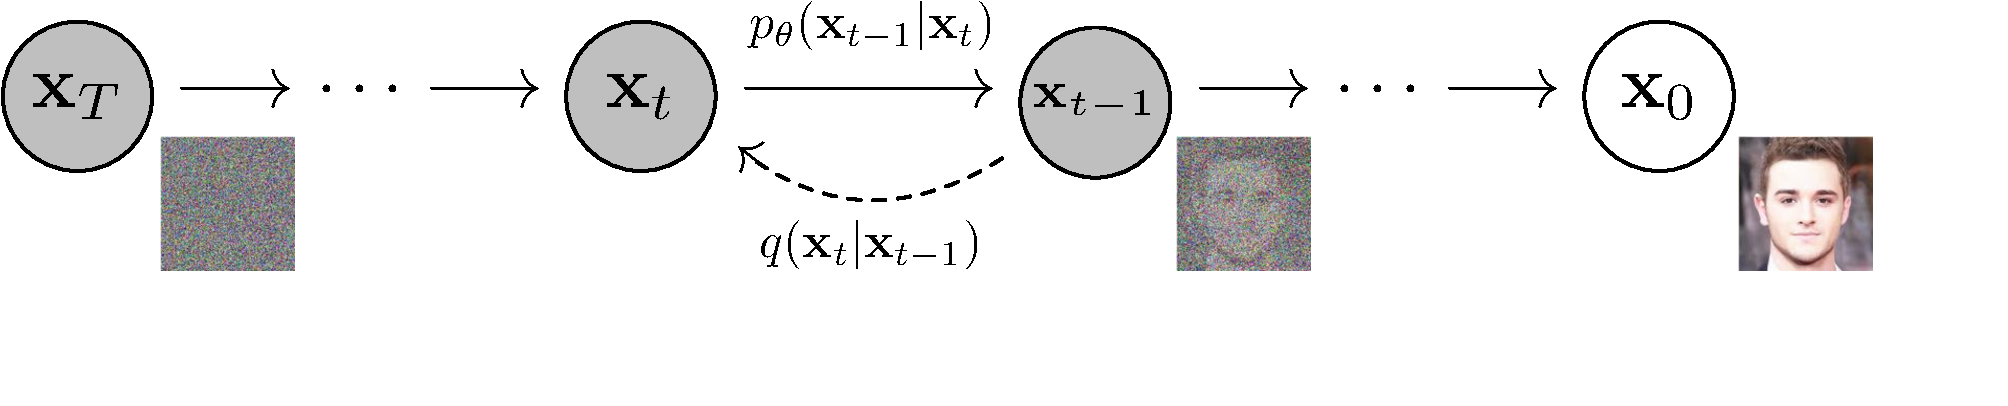
\includegraphics[width=0.99\textwidth]{figure/related/ddpm.pdf}
  \caption{基于扩散过程的图像去噪合成示意图\citep{Ho2020ddpm}。}
\end{figure}
近来,随着扩散模型本身理论不断成熟,越来越多的工作开始尝试在各类具体任务中使用扩散模型来利用其生成样本质量高的优点并试图改善其推理速度慢的问题。\citet{kong2021diffwave}~和\citet{chen2021wavegrad}~两篇工作尝试将扩散模型应用于构建神经声码器这样的模型,根据梅尔频谱生成高保真的声音波形。
\begin{figure}[!h]
  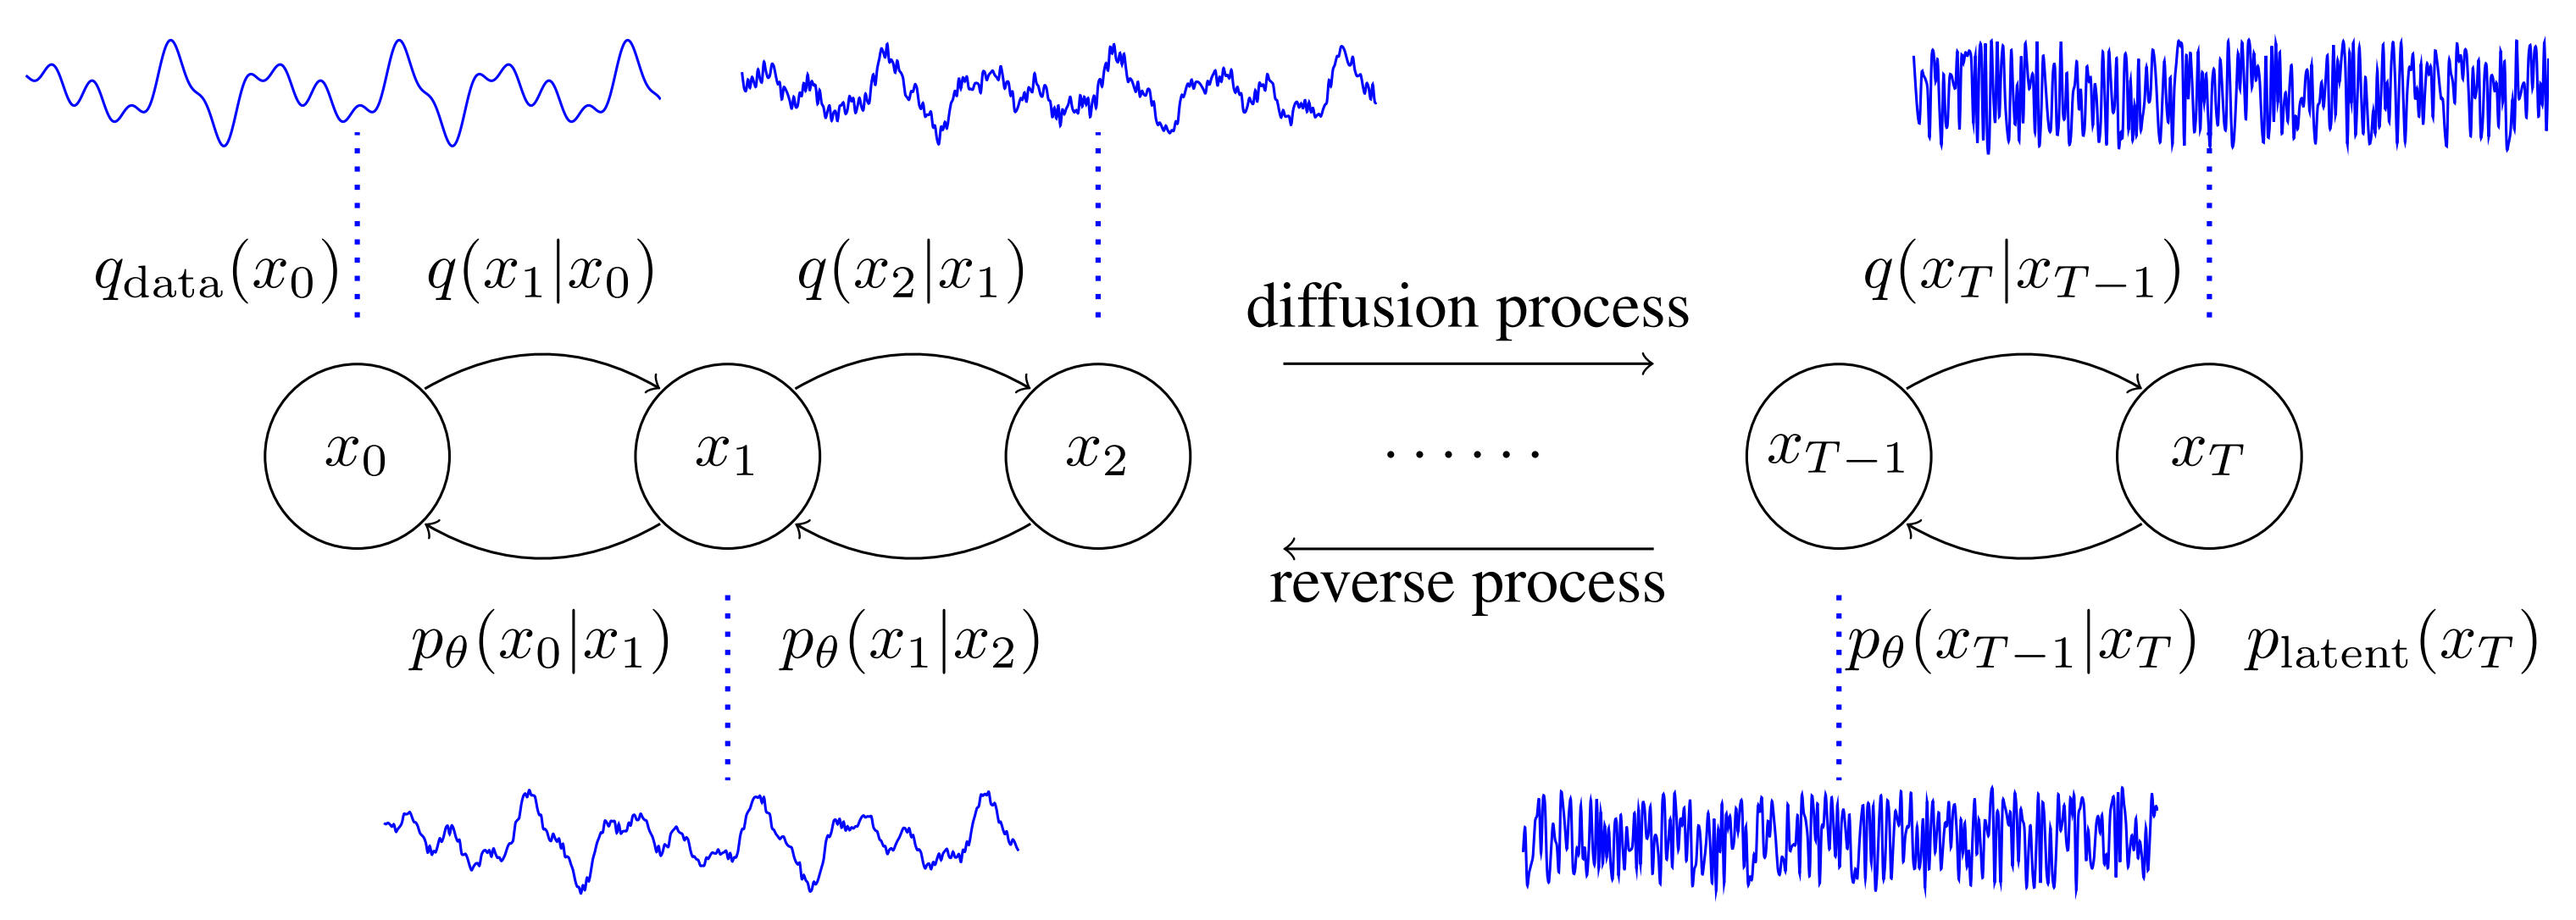
\includegraphics[width=0.99\textwidth]{figure/related/diffwave.png}
  \caption{基于扩散过程的声音波形合成示意图\citep{kong2021diffwave}。}
\end{figure}
后者同时还提出了一种连续的噪声时序变化函数来减少推理迭代所需要的时间步数来对推理进行加速,同时保持原有的合成质量。\citet{song2021denoising}~将扩散模型的理论统一到了得分匹配框架中,通过将随机微分方程近似为常微分方程的形式给出了更快的采样机制和在样本之间插值的方法。扩散模型是一种新兴的合成技术,已有成功应用于无条件图像生成、条件指导下的梅尔频谱到波形生成(神经声码器)等任务的多篇工作。在本文的工作中,第\ref{sec:svs}章提出了一个基于扩散模型声学模型用于进行翻唱歌曲的合成,该模型在给定乐谱和文本(或仅给定文本)的情况下生成相应的歌声梅尔频谱。
\section{本章小结}
本章主要分多个领域分别介绍了歌曲歌词生成及限制性翻译、歌词-旋律对齐预测、语音合成声学模型、歌声合成和扩散模型相关技术的背景、基本原理、国内外相关研究介绍和近期进展。

\newcommand{\modelname}{LTAG}
\chapter{自动歌曲翻译}
本章将详细介绍本文在自动歌曲翻译研究中使用的数据、提出的模型和实验结果。本章首先说明了使用的单语言数据集来源、收集双语平行数据集的方法,并提出一种基于神经机器翻译中常用的Transformer Encoder-Decoder结构的歌词和歌词-旋律对齐共同翻译框架,并在此基础上设计了一系列实验来检验模型框架的表现。实验结果显示,本章提出的框架相比其他自动歌曲翻译算法,在歌词文本翻译质量和歌曲翻译整体演唱效果上都取得了更好的效果。
\section{歌曲翻译数据集}
目前,在歌曲翻译研究领域并没有高质量的平行歌词翻译和歌词-旋律对齐的公共数据集可用,所以本文收集并标注了一个数据集PopCV(Pop songs with Cover Version),该数据集包含若干中文歌曲的英文翻唱版本和英文歌曲翻唱版本。除此以外,本文还使用了一些单语言歌曲语料, 包括一个英文歌词和歌词-旋律对齐数据集LMD\footnote{\url{https://github.com/yy1lab/Lyrics-Conditioned-Neural-Melody-Generation}}~\citep{LMD},以及一个从唱吧App上爬取的一些中文歌曲语料。
两组单语言歌曲数据仅被用于训练模型,测试数据是在经专业标注人员标注的真实数据上进行的。数据集概述见表\ref{tab:dataset_stat}.
\begin{table}[htbp]
    \centering
    % \setlength{\tabcolsep}{2pt}
    \begin{tabular}{|l|c|c|c|c|}
    \hline
         & 语种 & 歌曲数(首) & 歌词数(句) & 数据来源和实验用途\\
    \hline
     LMD & 英文 & \diagbox[]{}{} & 152,991 & 回译\\
    \hline
     唱吧 & 中文 & \diagbox[]{}{} & 542,034 & 回译\\
    \hline
     PopCV & 中文、英文 & 79 & 2,959 & 标注\\
    \hline
     测试集 & 中文、英文 & 25 & 629 & 标注\\
    \hline
    \end{tabular}
    \caption{本文中所涉及的数据集的数据统计情况。}
    \label{tab:dataset_stat}
\end{table}
\section{歌曲翻译数据的收集和预处理}
由于此类歌曲翻译的数据集并没有行业标准或其他公开发布的先例,于是,本文首先设计了一个相对省时且对于标注员来说,比较容易执行的标注过程。
首先,从一些公开的乐谱网站收集歌曲的乐谱文件\footnote{\url{https://www.musescore.com} 和 \url{https://wwww.midishow.com}}.
然后,专业标注人员会根据歌曲在原版和翻唱版本中的演唱方式,按照一般的歌谱编纂规则的指示\footnote{\url{https://lilypond.org} and \url{https://musescore.org/howto}}将歌词添加到乐谱的音符上。
然后,标注好的乐谱文件会被以\texttt{.musicxml}的格式导出,然后自动提取出歌词及其对齐的音符并整理成数据集。
\begin{figure}[t]
    \centering
    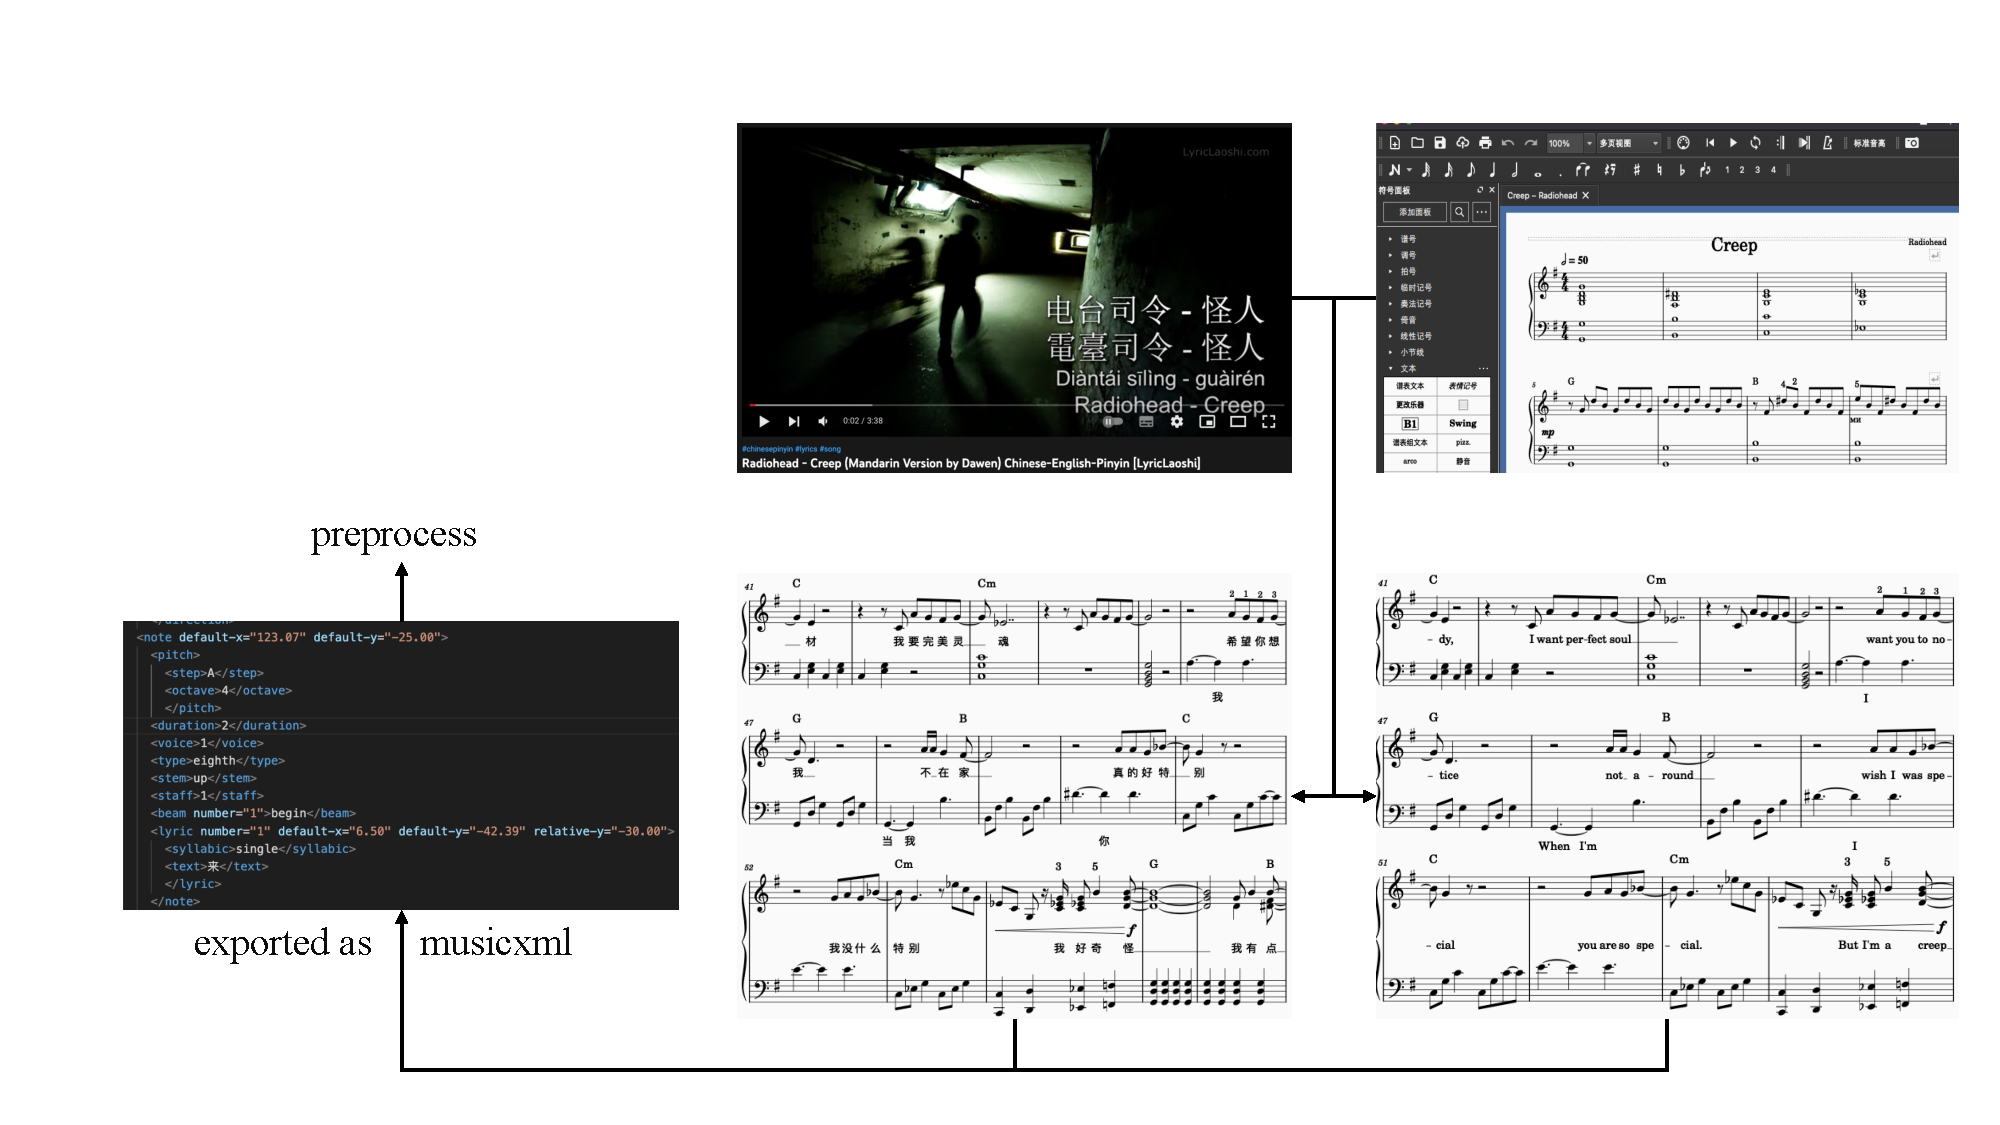
\includegraphics[width=0.99\textwidth]{figure/ast/da_pipeline}
    \caption{本文提出的歌曲翻译数据标注流程概览。}
    \label{fig:da_pipeline}
\end{figure}
\section{自动歌曲翻译模型结构}
本章设计的模型属于神经机器翻译中常用的自回归翻译架构,但与一般的翻译模型不同的是,它能同时进行自回归的歌词文本翻译和歌词文本与旋律的对齐预测。
如图\ref{fig:model}所示,它由用于歌词翻译的基于Transformer Encoder-Decoder的子结构、两个音符表示池化嵌入层和一个对齐解码器组成。
\begin{figure}[t]
    \centering
    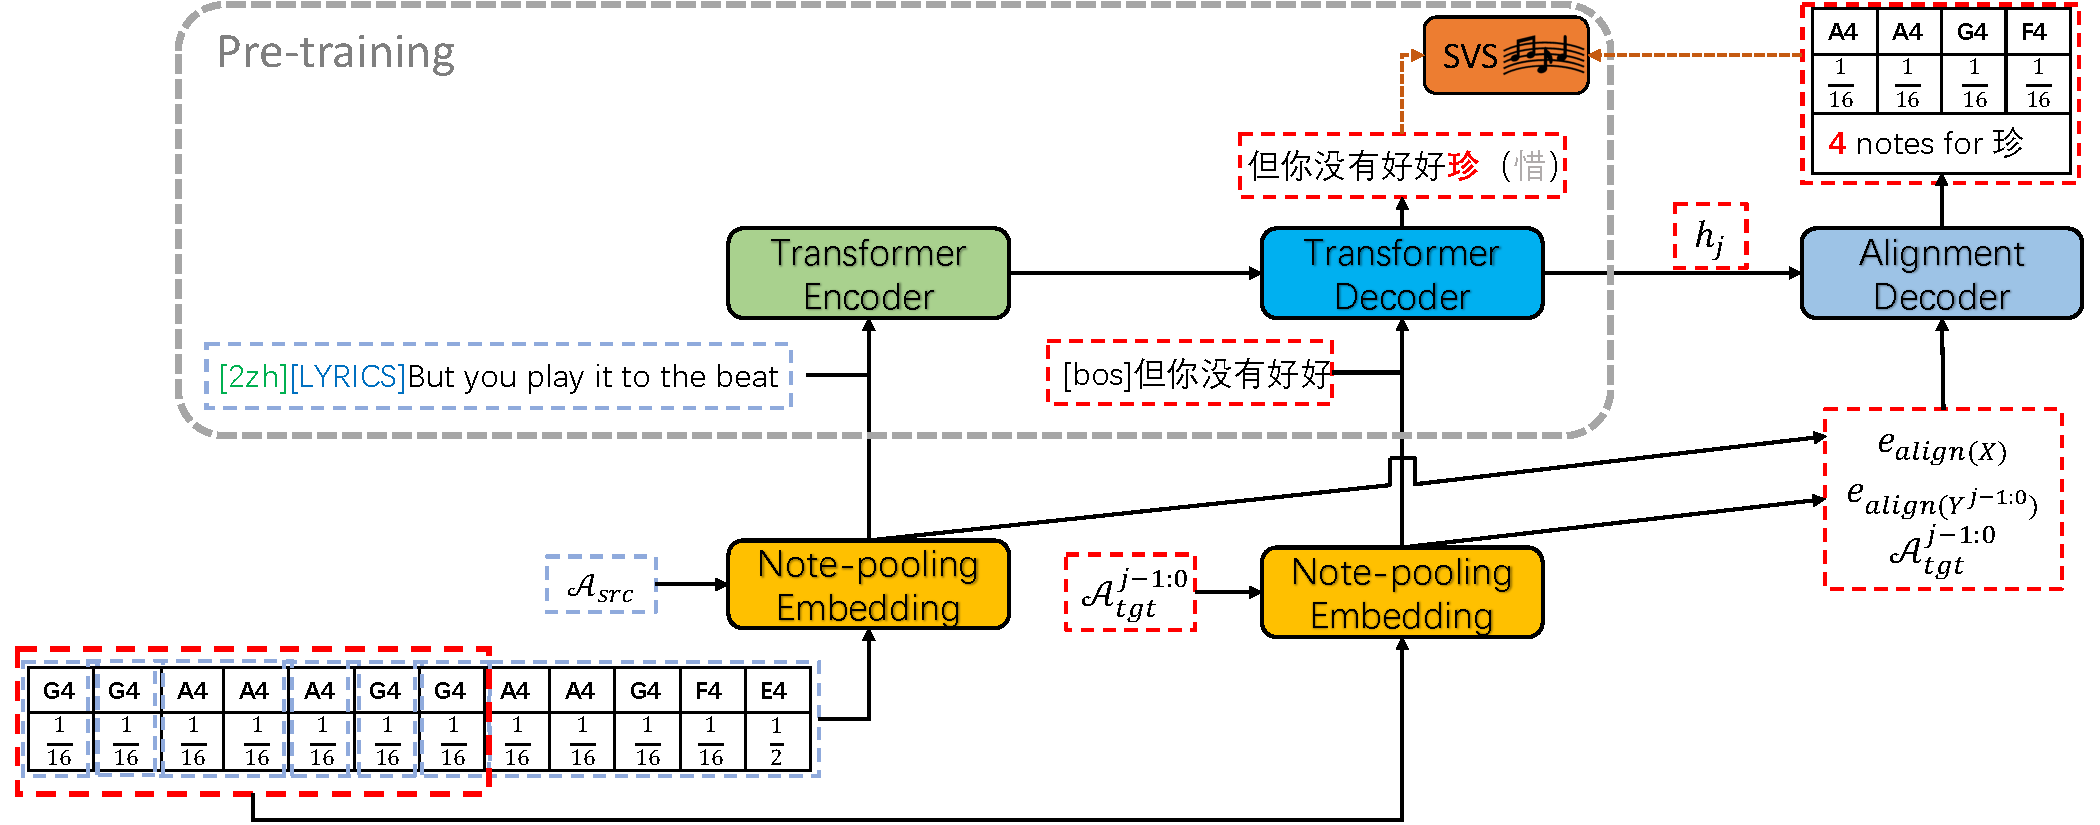
\includegraphics[width=0.99\textwidth]{figure/ast/pipeline_svs.pdf}
    \caption{本章提出的模型架构概览,图示以第$j$个解码时间步进行了说明。Transformer解码器将输出目标语言的词语,对齐解码器会输出对齐音符的数量。}
    \label{fig:model}
\end{figure}
Transformer Encoder-Decoder部分参考了\citet{gagast}中的做法,使用去噪自编码器~\citep{bart}和翻译作为预训练任务。
在预训练期间,由于混合使用了单语言和双语翻译数据,且数据文本来自新闻、书本和歌词等多个领域,两个分别表示翻译方向和文本域的前缀词语会被添加到源语言的输入句子里以建立模型区分翻译方向和目标文本所属文本域的能力。
音符表示池化嵌入层的结构如图~\ref{fig:align_enc}所示,这是一个用于处理歌曲旋律信息的模块。
图~\ref{fig:align_dec}中的对齐解码器则是基于本章后提出的节的自适应音符分组方法构建,该方法在自回归解码期间能动态预测与当前解码时间步预测出的的词语相对齐的音符数量。
\begin{figure}[t]
    \centering
\subfloat[The note-pooling embedding layer]{
    \label{fig:align_enc}
    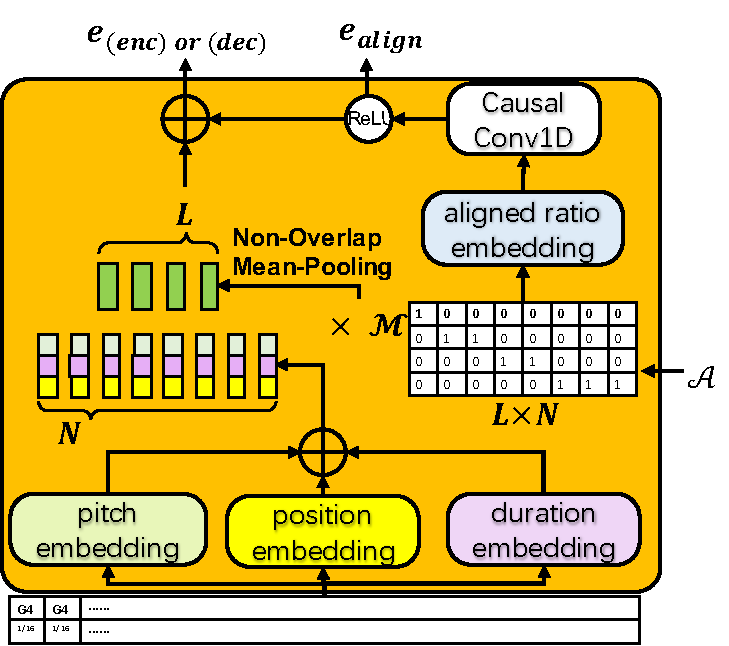
\includegraphics[width=0.34\textwidth,clip=true]{figure/ast/note-pooling.pdf}
}
\subfloat[The alignment decoder]{
    \label{fig:align_dec}
    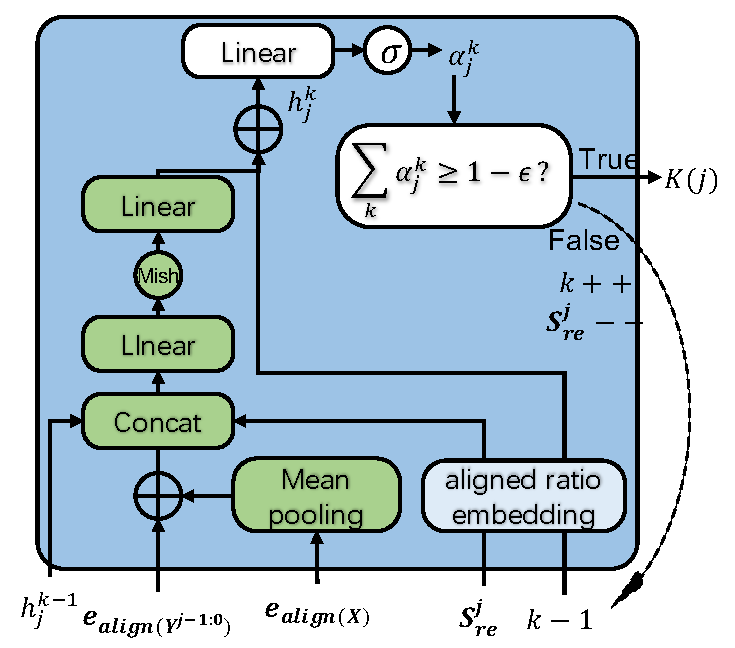
\includegraphics[width=0.31\textwidth,clip=true]{figure/ast/alignment_decoder.pdf}
}
\subfloat[Adaptive grouping process]{
    \label{fig:act_gp}
    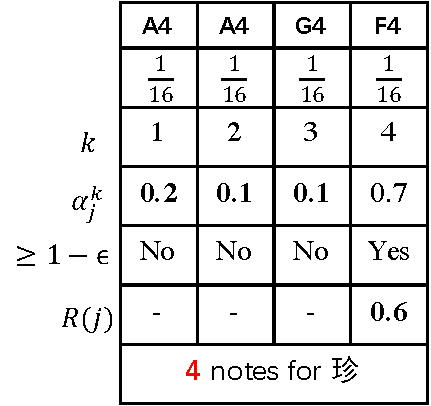
\includegraphics[width=0.28\textwidth,clip=true]{figure/ast/act_gp.pdf}
}
\caption{(a)音符表示池化嵌入层会根据音符序列的表示和对齐信息进行编码。(b)(c)对齐解码器会根据停止概率的分布计算对齐音符的数量。}
\label{fig:enc_dec_act}
\end{figure}
\subsection{音符表示池化嵌入层}
\label{sec:note_pooling}
音符表示池化嵌入层将音符和音符与歌词词语的对齐信息作为输入,并输出池化后的音符嵌入表示和对齐嵌入表示。
输入的旋律音符序列由MIDI格式的音高和每个音符的持续时间两部分组成。每一个音符的持续时间都是离散的谱面时长的一类:四分音符、半音符或八分音符等。
音符的MIDI音高和持续时间可以分别表示为嵌入表示$e_{midi}$和$e_{dur}$。
定义第$i$个音符的嵌入表示为:
\begin{equation}
\label{eq:note}
    \mathbf{e}_{note}^i = \mathbf{e}_{midi}^i + \mathbf{e}_{dur}^i + \mathbf{e}_p^i
\end{equation}
其中,$\mathbf{e}_p^i$是位置嵌入表示。
池化嵌入层会根据对齐信息,对音符的嵌入表示序列进行互不重叠的平均池化操作。具体而言,就是将对齐到同一词语的连续的一段音符序列的嵌入表示进行平均。下面给出公式化的表达,对齐信息$\mathcal{A}$会被表示为一个01矩阵$\mathbf{M} \in \{0,1\}^{L \times N}$,其中$L$和$N$分别表示文本序列和音符序列的序列长度。如果第$i$个音符对齐到了第$j$个词语,那么$\mathbf{M}_{ji}=1$,否则$\mathbf{M}_{ji}=0$。
这样,$\mathbf{M}$就能直接通过矩阵乘法有效地进行互不重叠的平均池化操作,其结果记为为旋律嵌入表示$\mathbf{e}_{md}$。
\begin{equation}
\label{eq:md_embed}
    \mathbf{e}_{md} = \text{Non-Overlap-Mean-Pool}(\mathbf{e}_{note}, \mathbf{M})
\end{equation}
有音符嵌入表示$\mathbf{e}_{note} \in \mathbb{R}^{N \times d}$($d$ 是嵌入表示张量的维度)和对齐矩阵$\mathbf{M} \in \{0, 1\}^{L \times N}$.
互不重叠的平均池化操作可以按照如下计算进行:
\begin{align*}
\mathbf{W} &= \mathbf{M} / \text{sum}(\mathbf{M}, \text{dim}=-1, \text{keepdim}=\text{True}) \\
\mathbf{e}_{md} &= \mathbf{W} * \mathbf{e}_{note}
\end{align*}
其中,$/$代表矩阵按元素相除,$*$代表矩阵相乘。
通过pytorch支持的\texttt{gather}和\texttt{scatter}张量操作,上述互不重叠的平均池化操作就可以在训练时的小批次数据中进行了。
由上述说明易知,此池化操作的核的尺寸大小不是固定的,而是随着01矩阵$\mathbf{M}$的行的和变化而变化。

进一步说,由于歌词-旋律的对齐是单调的,即歌谱中每个音符只能对应一个词语,通过计算对齐音符的数量的累积和就可以更简洁地编码对齐情况:
\begin{equation}
\label{eq:cumsum}
    \mathbf{s} = \text{CumSum}(\text{RowSum}(\mathbf{M}))
\end{equation}
其中,$\mathbf{s}$是一个长度为$L$的整数向量。那么$s^j / N$就表示每个对齐音符的\textbf{对齐比率}。
接下来,通过将累积对齐比率分组为$(0,1]$范围内的大小相等的区间就可以将比率离散化,并引入一组嵌入表示张量$\mathbf{E}_{ratio}$来表示每个区间。划分成的区间数是一个可调节的超参数。所以,对齐比率嵌入表示的计算方法如下:
\begin{align}
\label{eq:align}
    \mathbf{e}_{align}^j = f(\mathbf{E}_{ratio}(s^j / N))
\end{align}
其中,$f(\cdot)$是一个简单的非线性神经网络层,由一维因果卷积层和ReLU激活函数组成。
最后,将旋律嵌入表示和对齐比率嵌入求和,结果被输入到基于Transformer的子结构的编码器或解码器,和其中原有的嵌入表示相加:
\begin{equation}
\label{eq:embed}
    \mathbf{e}_{\text{enc(dec)}} = \mathbf{e}_{token} + \mathbf{e}_p + (\mathbf{e}_{md} + \mathbf{e}_{align})
\end{equation}
如公式~(\ref{eq:md_embed})所示,每个旋律嵌入表示都会对应于该段旋律对齐到的词语。
此外,使用因果卷积层意味着音符对齐比率的嵌入张量也具有与文本序列相同的长度,并且能够保证每个对齐比率的嵌入表示仅以自回归的方式与先前的比率嵌入表示相关。上述性质就保证了该层在解码器中可以完美地适应自回归方式的翻译需要进行的Teacher-forcing式训练。
来自源端歌词的对齐嵌入表示由于在解码时并没有目标端的词语可以对去,所以这部分会整体经过池化层处理以形成全局的对齐参考表示,并输入到对齐解码器中。
本章提出的这种设计的动机在于用对齐的音符数来隐式地对歌词的翻译过程进行限制。

\subsection{对齐解码器的结构}
受自适应计算时间方法(Adaptive Computation Time,ACT)~\citep{act}的启发,本章提出了\textbf{自适应分组}模块来对歌词和音符的对齐情况进行建模。
如图\ref{fig:align_dec},\ref{fig:act_gp}所示,此模块能够预测出应将多少个连续的音符分配给当前解码时间步正在处理的词语。
\subsubsection{自适应音符分组预测}
一般地,有$1 \leq j \leq L_Y$,设$y_j$为第$j$个目标端文本词语,$\mathbf{h}_j$为基于Transformer的解码器的最后一层相对应的隐层表示。
为了说明之便而又不失一般性,假设之前的文本序列$y_{j-1:0}$已经与前$n-1$个音符完成对齐,下文将通过遍历一个索引变量$k$($k$从1开始)来定义自适应音符分组预测与$y_j$对齐的音符数量的过程。
\begin{align}
    \mathcal{S}_{re}^j &= N -s^{j-1}_{tgt} \\
     \mathbf{h}_j^0 &= \mathbf{h}_j  \\
     \mathbf{h}_j^k &= g(\mathbf{h}_j^{k-1}, \mathbf{e}_{align(X)}, \mathbf{h}_{align(y_{j-1:0})}, \mathcal{S}_{re}^j, k-1) \\
     \alpha_j^k &= \sigma(\text{Linear}(\mathbf{h}_j^k))
\end{align}
其中,$\mathbf{e}_{align(X)}$是完整的来自源语言端的对齐嵌入表示,$\mathbf{e}_{align(y_{j-1:0})}$则是已经过解码的先前部分的对齐嵌入表示,$s^{j-1}_{tgt}$是$\mathbf{s}$向量中的第$j$元素($\mathbf{s}$来自公式~(\ref{eq:cumsum})。
现在模型既有每句歌词对应的完整旋律中的音符数量信息,又有已经对齐到目标端的音符数量,那么可以计算当前解码步骤中第$j$时间步时,剩余未对齐音符的数量为$\mathcal{S}_{re}^j$。如上文所述,$\mathbf{e}_{align(X)}$经过一个平均池化层以获得单个向量表示作为全局参考,从而使得来自源语言端的对齐情况始终可以与可变长度的目标端的$\mathbf{e}_{align(y_{j-1:0})}$进行加和。
一个多层神经网络$g(\cdot)$会对所有的输入进行处理,具体网络结构如图\ref{fig:align_dec}中绿色部分所示。
最后,经Sigmoid函数$\sigma(\cdot)$处理,模块会这一步处理中间态的自适应分组停止概率$\alpha_j^k$。
所有中间态停止概率的总和表示当前$k$个音符与目标端词语$y_j$对齐的可能性。

给定一个超参数$\epsilon$,通常为一个很小的浮点数(例如,0.01),如果此时的$k$满足$\sum_k \alpha_j^k < 1-\epsilon$,即累计概率未超过阈值,那么自适应分组过程会继续进行并将$k$递增为$k=k+1$;相应递减$\mathcal{S}_{re}^j=\mathcal{S}_{re}^j-1$,然后进行上述计算。
否则,累计概率已经超过了既定阈值,对齐预测的分组过程停止,对齐解码器输出当前对齐的音符数$K(j)$。
\begin{equation}
\label{eq:Kj}
    K(j) = \underset{K}{\mathrm{argmin}} \left\{\sum_{k=1}^K \alpha_j^k \geq 1-\epsilon \right\}
\end{equation}

在$\epsilon$是正值$\epsilon>0$的情况下,这个预测过程能确保$K(j)\geq1$,也就是说对于每个词语,至少有一个音符会被对齐到该词语上。
为了清晰地定义对齐$K(j)$个音符到当前词语的概率,引入一个余项$R(j) = 1-\sum_{k=1}^{K(j)-1} \alpha_j^k$。
这样,$\alpha_j^k$和$R(j)$就都可以是有效的概率分布了。
图\ref{fig:act_gp}是本节提出的自适应分组方法在歌词音符对齐预测上运行的一个示例。

\begin{equation}
\begin{array}{rl}
    L_G = & \left| \sum_j K(j) - N \right| + \sum_j \left|K(j) - \Delta_j\right| \\
    \approx &\left|\sum_j \left(K(j) - (1 - R(j))\right) - N \right| \\
    & + \sum_j \left|K(j) - (1 - R(j)) - \Delta_j\right|
\end{array}
\end{equation}
\subsubsection{自适应分组模块的梯度计算}


\section{基于Back Translation的数据增强}
\label{sec:bta}
虽然本章中收集的规模在上千句左右的歌曲数据集能够初步满足训练模型的需求,其中包含的来自人工翻译平行双语歌词和歌词-旋律对齐信息的标注数量是非常有限的,而且这对标注人员素质提也提出了较高要求,因此对于实际应用会有收集耗时较长,代价昂贵的问题。

所以,本章还改造了近年来神经机器翻译研究中广泛使用的基于回译的数据增强方法\citep{backtrans}来生成更多的双语歌曲训练数据。
相比于本章提出的人工标注的平行双语歌曲数据集,在公开网络上显然可以搜集到数量更为庞大的单语歌曲数据。通过构建一个可以进行长度控制的预训练歌词翻译模型,目标语言中的单语数据就能被回译到源语言中。
长度控制可以确保翻译出的结果的词语的数量与所对应的旋律的音符数量相同,这样就能在源语言端制造歌词和音符的简单一对一对齐。
经过如此改造后的回译方法就能够制造出相对较大的双语歌曲数据集。显然,这样增强出的数据在源端有信息噪声,但在目标端仍然保留了非常准确的信息。
由于回译出的数据比人工标注的数规模大得多,本章在实际训练中采用了类似课程学习的方式来进行训练时的数据采样。即在训练初期,来自回译增强的数据将与来自人工标注的数据真实数据混合。人工标注的数据被上采样到与回译数据差不多的数量级,
对回译数据的降采样率则会随训练进行不断减小,这样,每个小批次训练数据中人工标注数据的占比就会随着训练的进行不断提高。

\section{损失函数对于自动歌曲翻译模型的优化}
\section{歌曲翻译的评价指标}
对本章提出的模型所针对的自动歌曲翻译任务的表现的评价,最有说服力的指标就是翻译后的歌曲结果是否能被正常演唱、歌词文本易于理解,以及,最核心的指标,是否仍和原歌曲一样是人类乐于欣赏的歌曲作品。
因此,本章的实验评测参考了\citet{songmass}~中的做法:在进行人工评测时,评测人员会根据展示出的模型翻译结果——歌词和歌词-旋律对齐情况制成的歌谱,给出评测打分。

但是由于本章针对的自动歌曲翻译任务的特殊性,为了以一种接近实际中端到端的方式验证翻译结果的可唱性,本章的实验评测还使用了一个开源的歌唱语音合成模型~\citep{diffsinger}为评测人员提供翻译后歌曲的演唱音频,期望以此让标注人员进行更直观的演唱评测。


客观翻译BLEU,主观MOS,对齐情况Alignment Score。
\begin{equation}
    % \text{AS} = \frac{\sum_{k} \min(\text{freq}_{pred}^k, \text{freq}_{gt}^k) * k)}{\sum_{k} \text{freq}_{gt}^k * k }
    \text{AS} = \frac{\sum_{k}\min(\text{freq}_{pred}^k/F_{pred}, \text{freq}_{gt}^k/F_{gt}) * k)}{\sum_{k} (\text{freq}_{gt}^k/F_{gt}) * k) }
\end{equation}
\section{实验设计}

\section{实验结果与分析}
\begin{table}[t]
    \centering
    %\setlength{\tabcolsep}{4pt}
    \begin{tabular}{l|c|c|c|c|c|c}
    \hline
    \multirow{2}{*}{模型名称} & \multicolumn{2}{c|}{MOS-T} & \multicolumn{2}{c|}{MOS-S} & \multicolumn{2}{c}{MOS-Q} \\
    \cline{2-7}
    & En$\rightarrow$Zh & Zh$\rightarrow$En & En$\rightarrow$Zh & Zh$\rightarrow$En$^\dagger$ & En$\rightarrow$Zh & Zh$\rightarrow$En$^\dagger$ \\
    \hline\hline
    GagaST & 3.66 $\pm$ 0.06 & 3.72 $\pm$ 0.05 & 3.49 $\pm$ 0.10 & \multirow{7}{*}{\diagbox[height=25pt, width=0.05\textwidth]{}{}} & 3.65 $\pm$ 0.05 & \multirow{7}{*}{\diagbox[height=25pt, width=0.05\textwidth]{}{}}\\
    \cline{1-4} \cline{6-6}
    \modelname-cls  & 3.66 $\pm$ 0.05& 3.79 $\pm$ 0.05 & 3.58 $\pm$ 0.07& & 3.62 $\pm$ 0.05& \\
    ~~~ only bt & 3.69 $\pm$ 0.05 & 3.80 $\pm$ 0.04 & 3.53 $\pm$ 0.09 & & 3.63 $\pm$ 0.05&\\
    ~~~ w/o bt & 3.64 $\pm$ 0.05 & 3.30 $\pm$ 0.05 & 2.16 $\pm$ 0.05 & & 3.14 $\pm$ 0.04 &\\
    \cline{1-4} \cline{6-6}
    \modelname  & 3.71 $\pm$ 0.05& 3.85 $\pm$ 0.05 & 3.68 $\pm$ 0.05&  & 3.69 $\pm$ 0.04&\\
    ~~~ only bt & 3.71 $\pm$ 0.05 & 3.80 $\pm$ 0.05 & 3.58 $\pm$ 0.07 & & 3.65 $\pm$ 0.04&\\
    ~~~ w/o bt  & 3.69 $\pm$ 0.05 & 3.28 $\pm$ 0.04 & 3.63 $\pm$ 0.07 & & 3.67 $\pm$ 0.04&\\
    % \midrule
    % \modelname~w/o bt  & & & & & & \\
    % \modelname~only bt & & & & & & \\
    % \modelname~+ bt  & & & & & & \\
    \hline
    \end{tabular}
    \caption{The Mean Opinion Score in translation intelligibility and naturalness~(MOS-T), singability~(MOS-S) and overall quality~(MOS-Q) with 95\% confidence intervals. The translation direction with $^\dagger$ means that audio samples of the translated song for evaluation are generated with the voice synthesis model that is not trained for that target language. So those results are presented in Appendix \ref{appendix:zh-en} and for reference only.}
    %带*的结果仅供参考
    \label{tab:subjective}
\end{table}


\begin{table}[tbp]
    \centering
    \begin{tabular}{l|c|c|c|c}
    \hline
    \multirow{2}{*}{模型名称} & \multicolumn{2}{c|}{BLEU$\uparrow$} & \multicolumn{2}{c}{AS. $\uparrow$}\\
    \cline{2-5}
    & En$\rightarrow$Zh & Zh$\rightarrow$En & En$\rightarrow$Zh & Zh$\rightarrow$En \\
    \hline\hline
    GagaST & 11.87 & 5.67 & 0.701 & 0.468\\
    \hline
    \modelname-cls & 14.21 & 10.01 & 0.827 & 0.555\\
    ~~~ only bt  & 15.54 & 10.21 & 0.709 & 0.667\\
    ~~~ w/o bt & 13.73 & 8.26 & 0.704 & 0.490 \\
    \hline
    \modelname & 16.02* & \textbf{10.68} & \textbf{0.923} & \textbf{0.781} \\
    ~~~ only bt  & \textbf{16.27} & 10.26* & 0.880* & 0.718* \\
    ~~~ w/o bt & 14.12 & 7.86 & 0.845 & 0.710\\
    ~~~ w/o $\mathbf{e}_{align}$  & 15.16 & 9.24 & 0.852 & 0.703\\
    \hline
    \end{tabular}
    \caption{两个翻译方向上的saceBLEU和对齐分数。*表示行内第二优的结果。}
    \label{tab:objective}
\end{table}

\begin{figure}[t]
    \centering
\subfloat[源歌谱和参考翻译结果 左图:英$\rightarrow$中。 右图: 中$\rightarrow$英。]{
    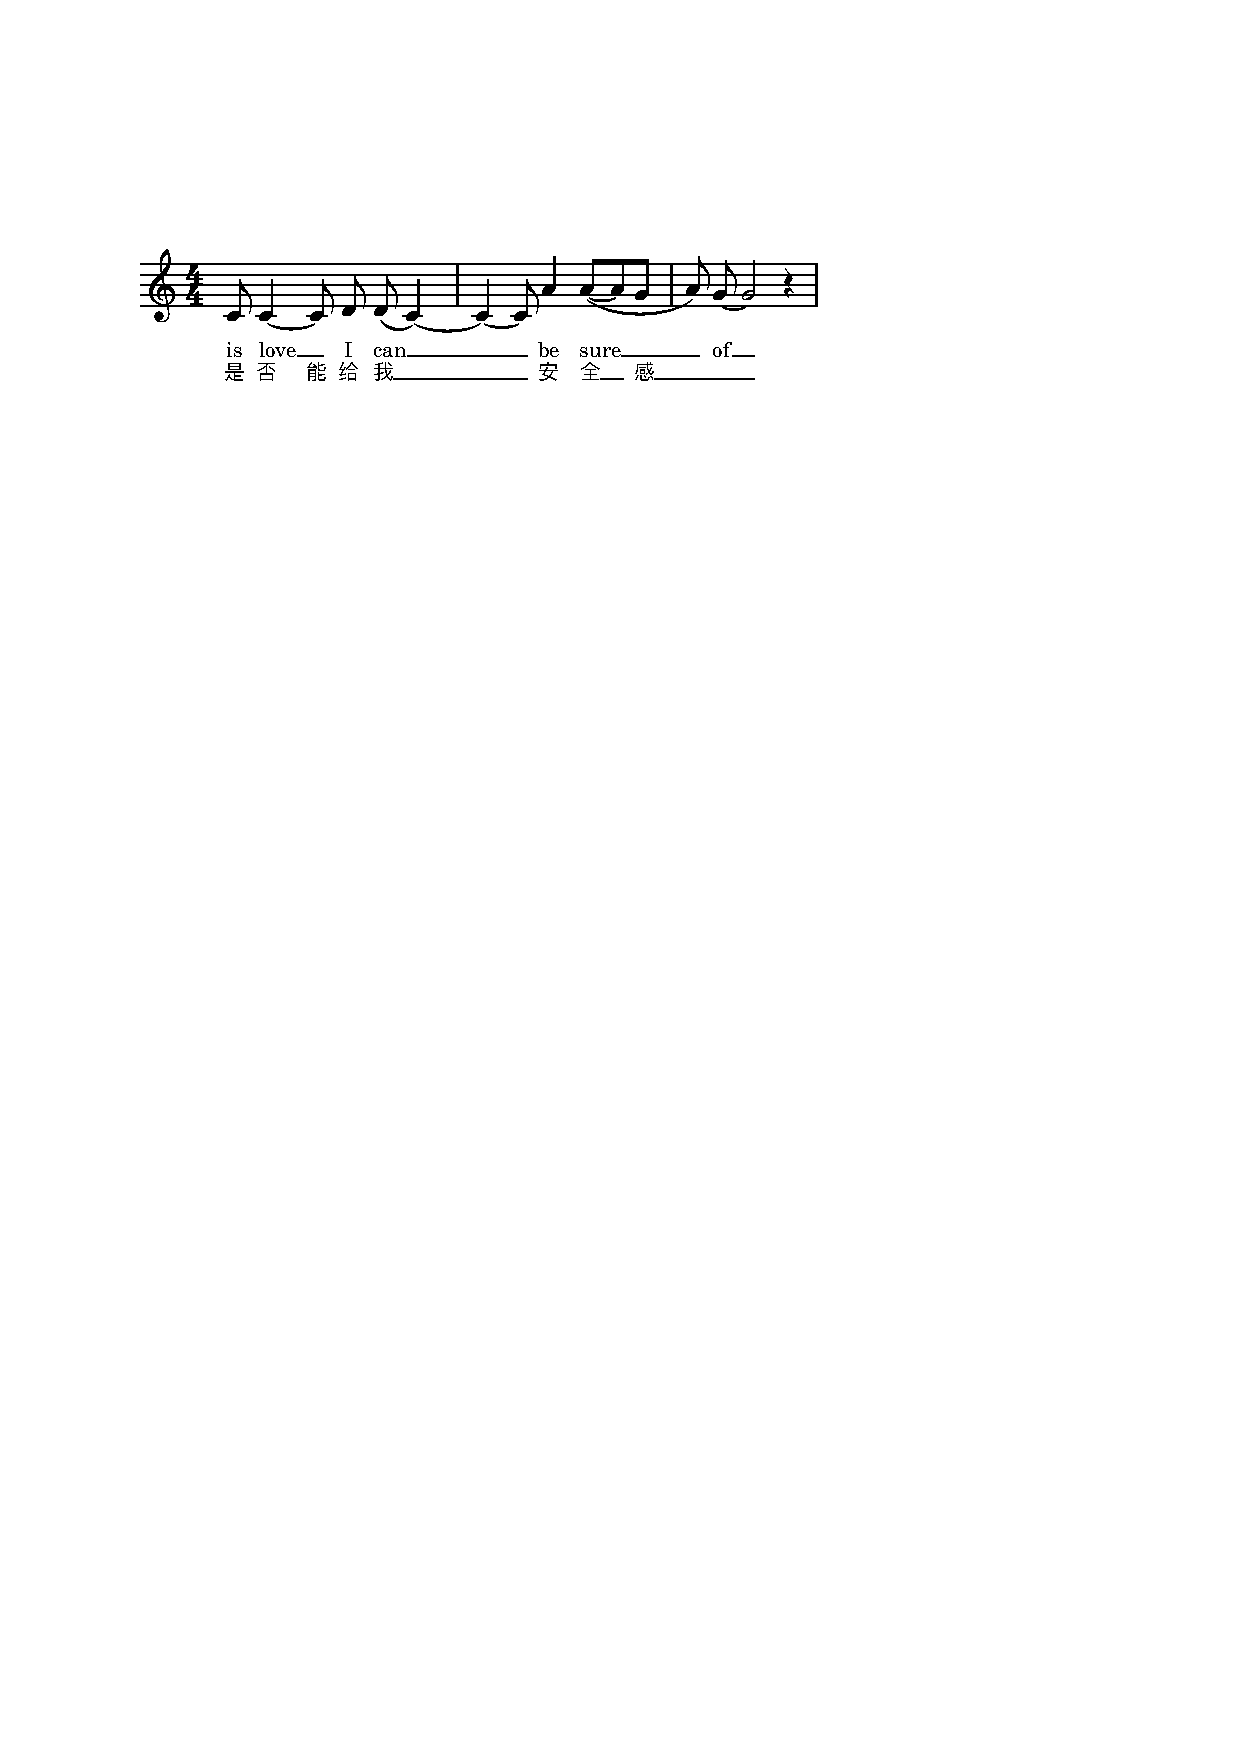
\includegraphics[width=0.55\textwidth,clip=true]{figure/ast/analysis_cases/exp_en_1.pdf}
    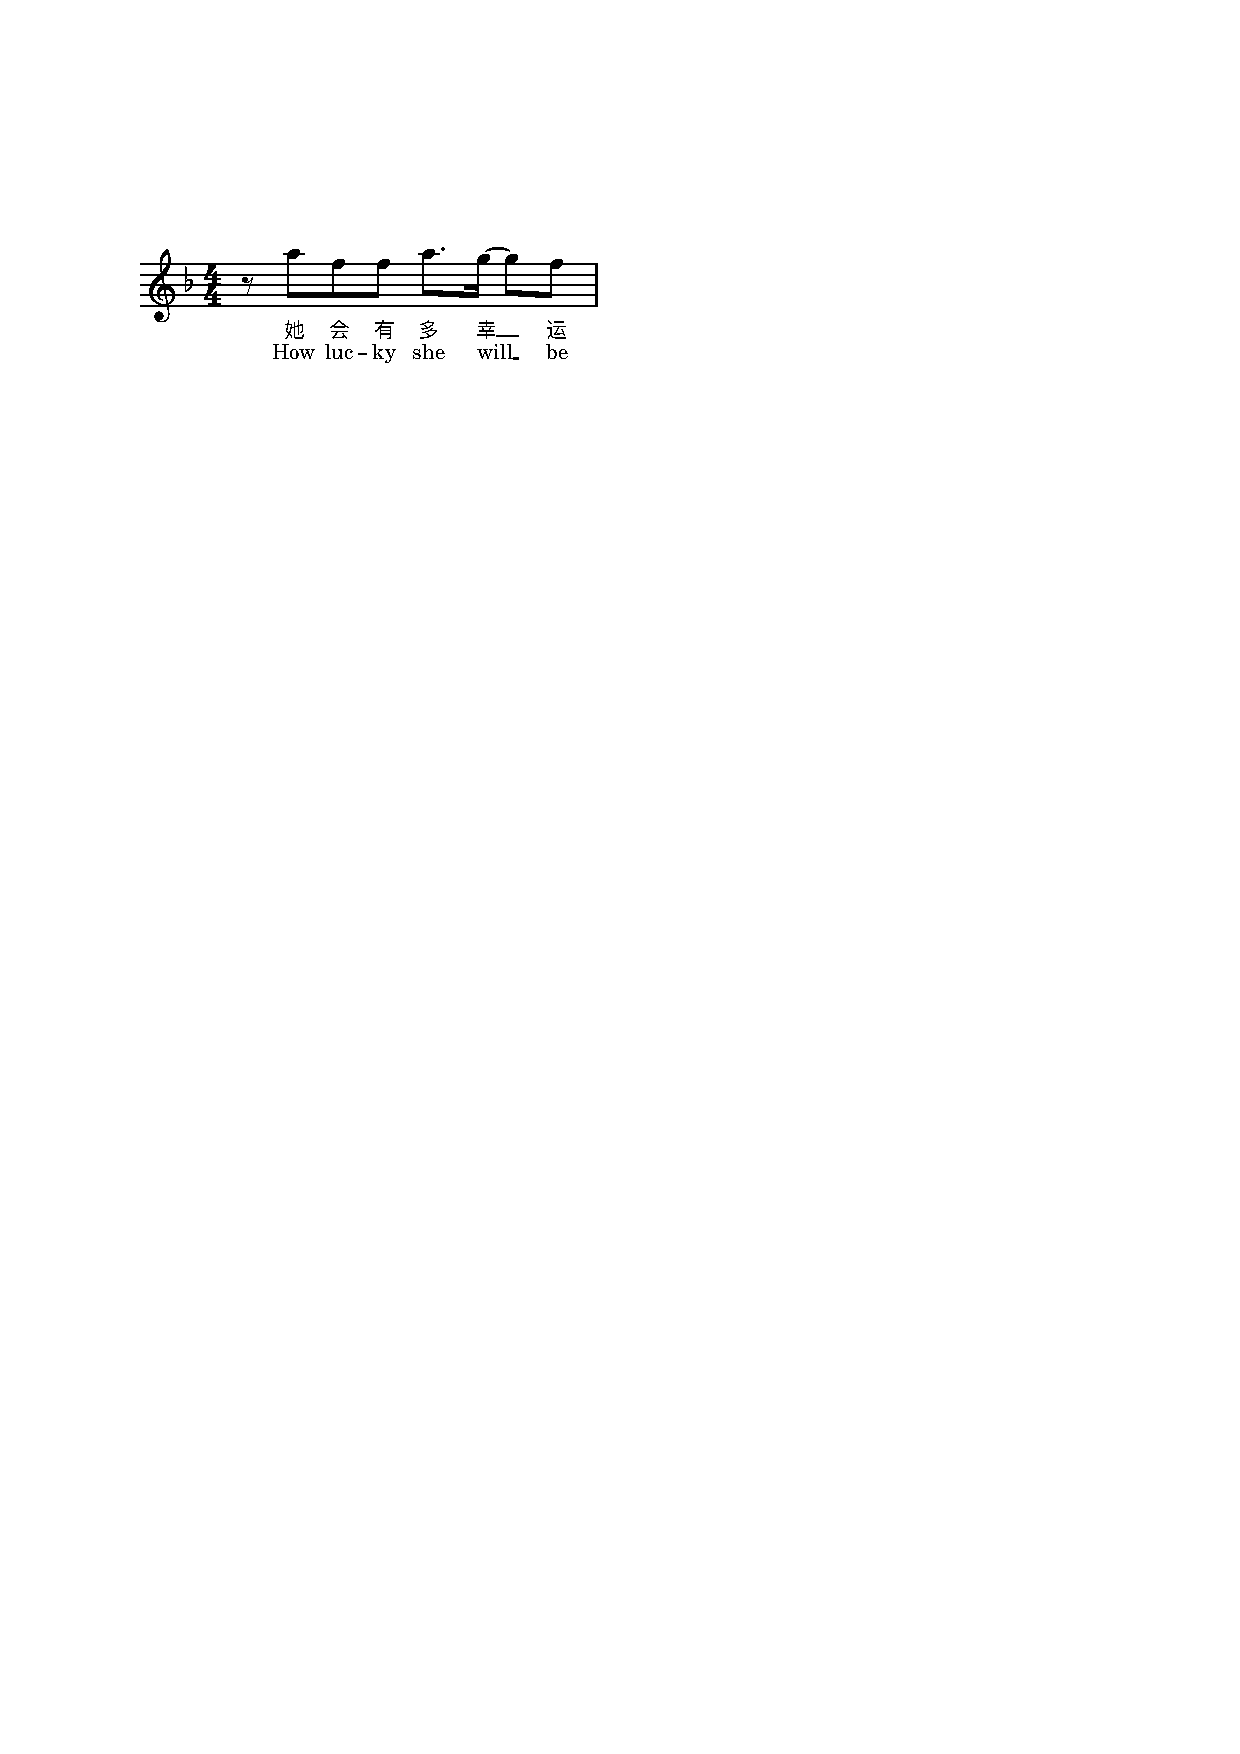
\includegraphics[width=0.43\textwidth,clip=true]{figure/ast/analysis_cases/exp_zh_2.pdf}
}\\
\subfloat[GagaST]{
    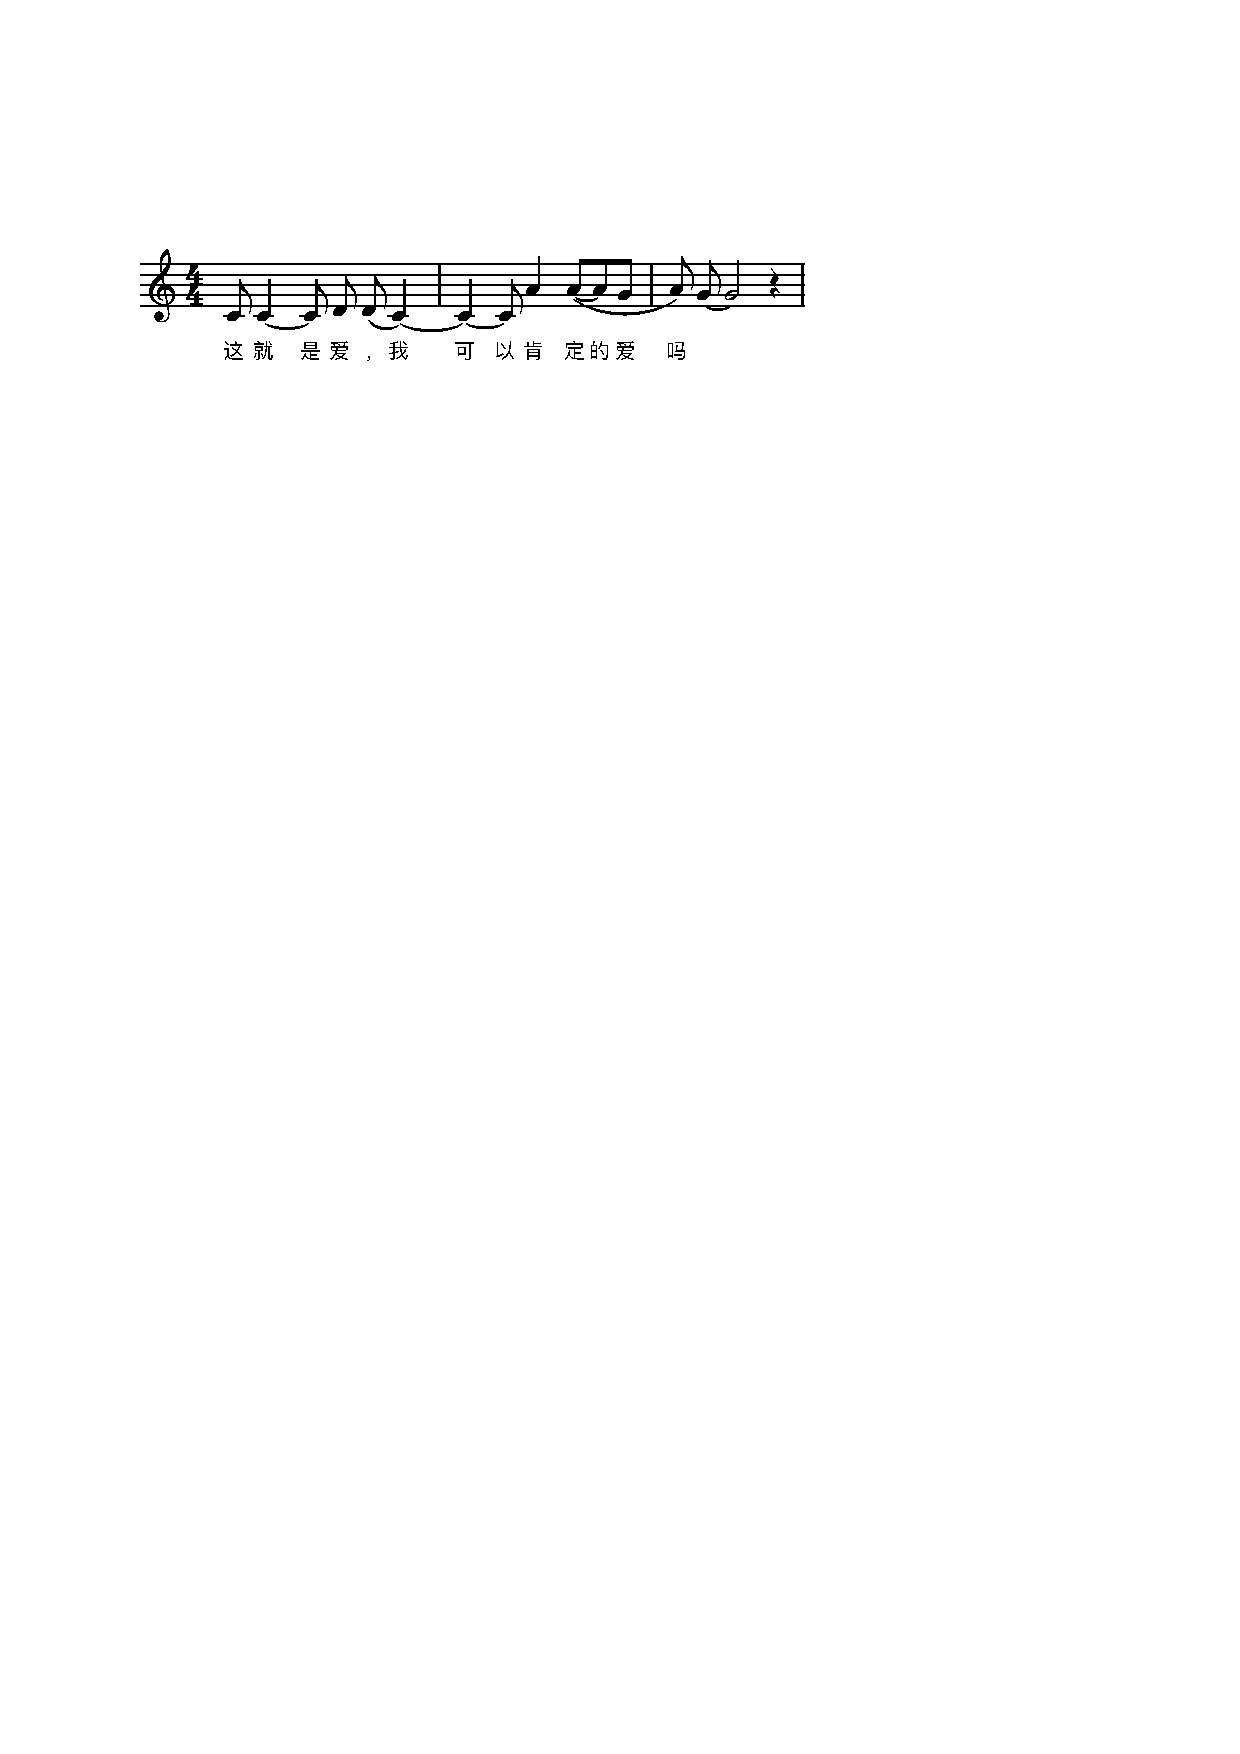
\includegraphics[width=0.55\textwidth,clip=true]{figure/ast/analysis_cases/exp_gagast_zh_1.pdf}
    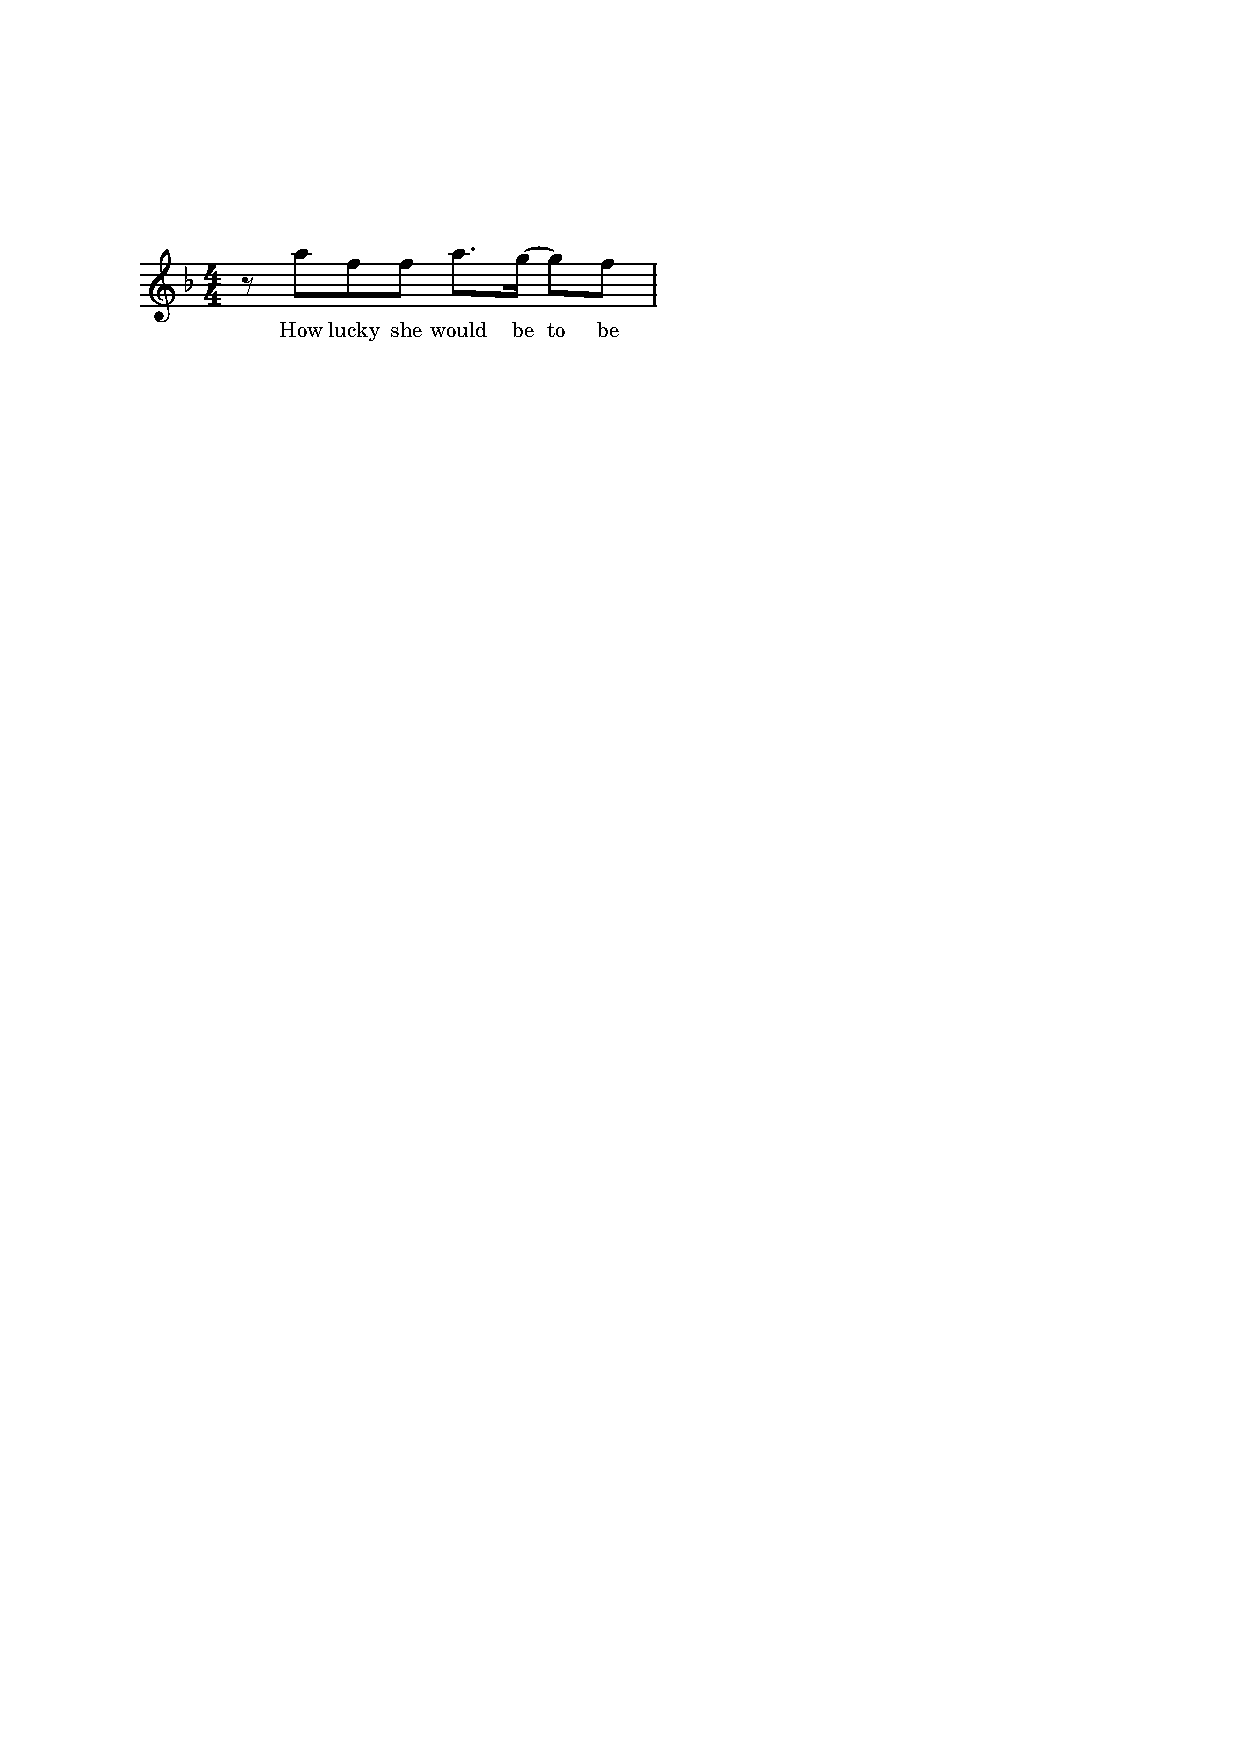
\includegraphics[width=0.44\textwidth,clip=true]{figure/ast/analysis_cases/exp_gagast_en_2.pdf}
}\\
\subfloat[\modelname-cls]{
    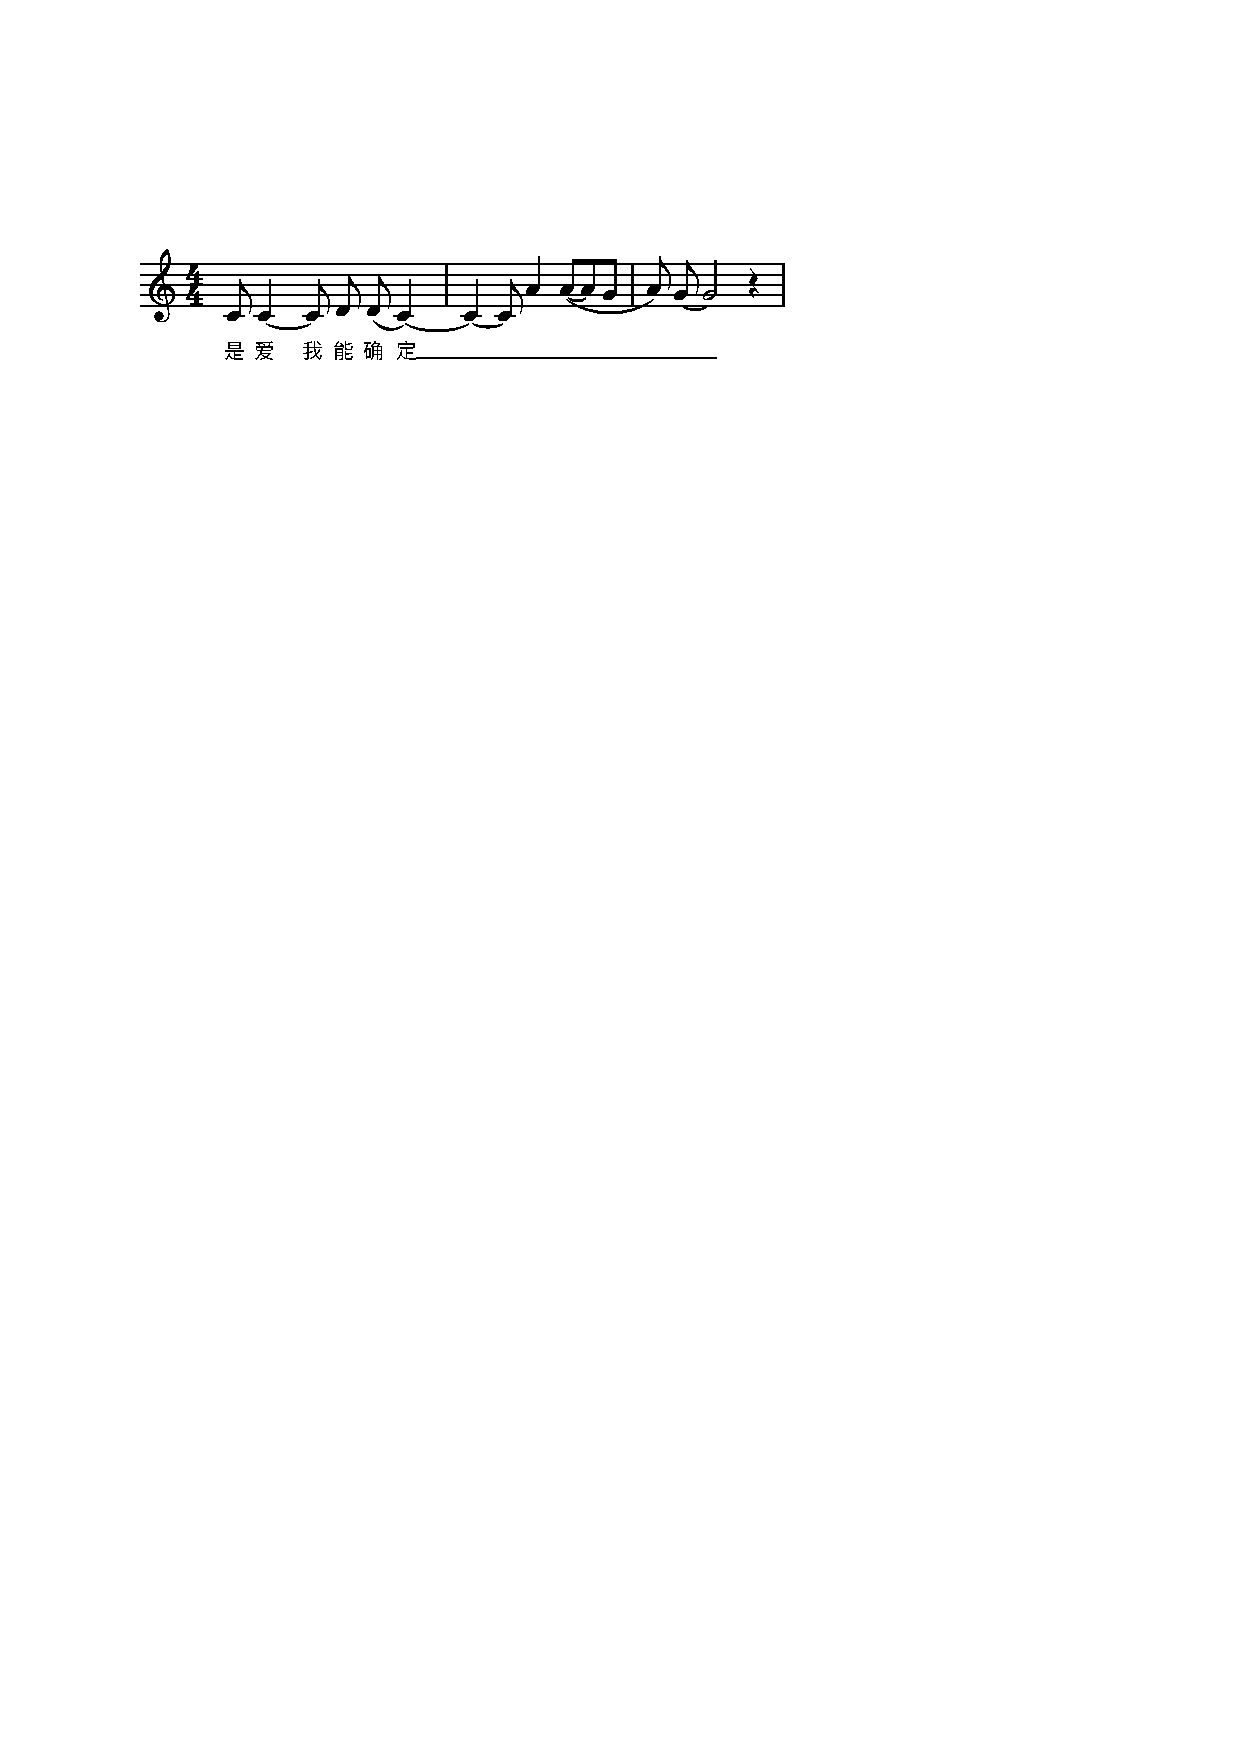
\includegraphics[width=0.55\textwidth,clip=true]{figure/ast/analysis_cases/exp_baseline_zh_1.pdf}
    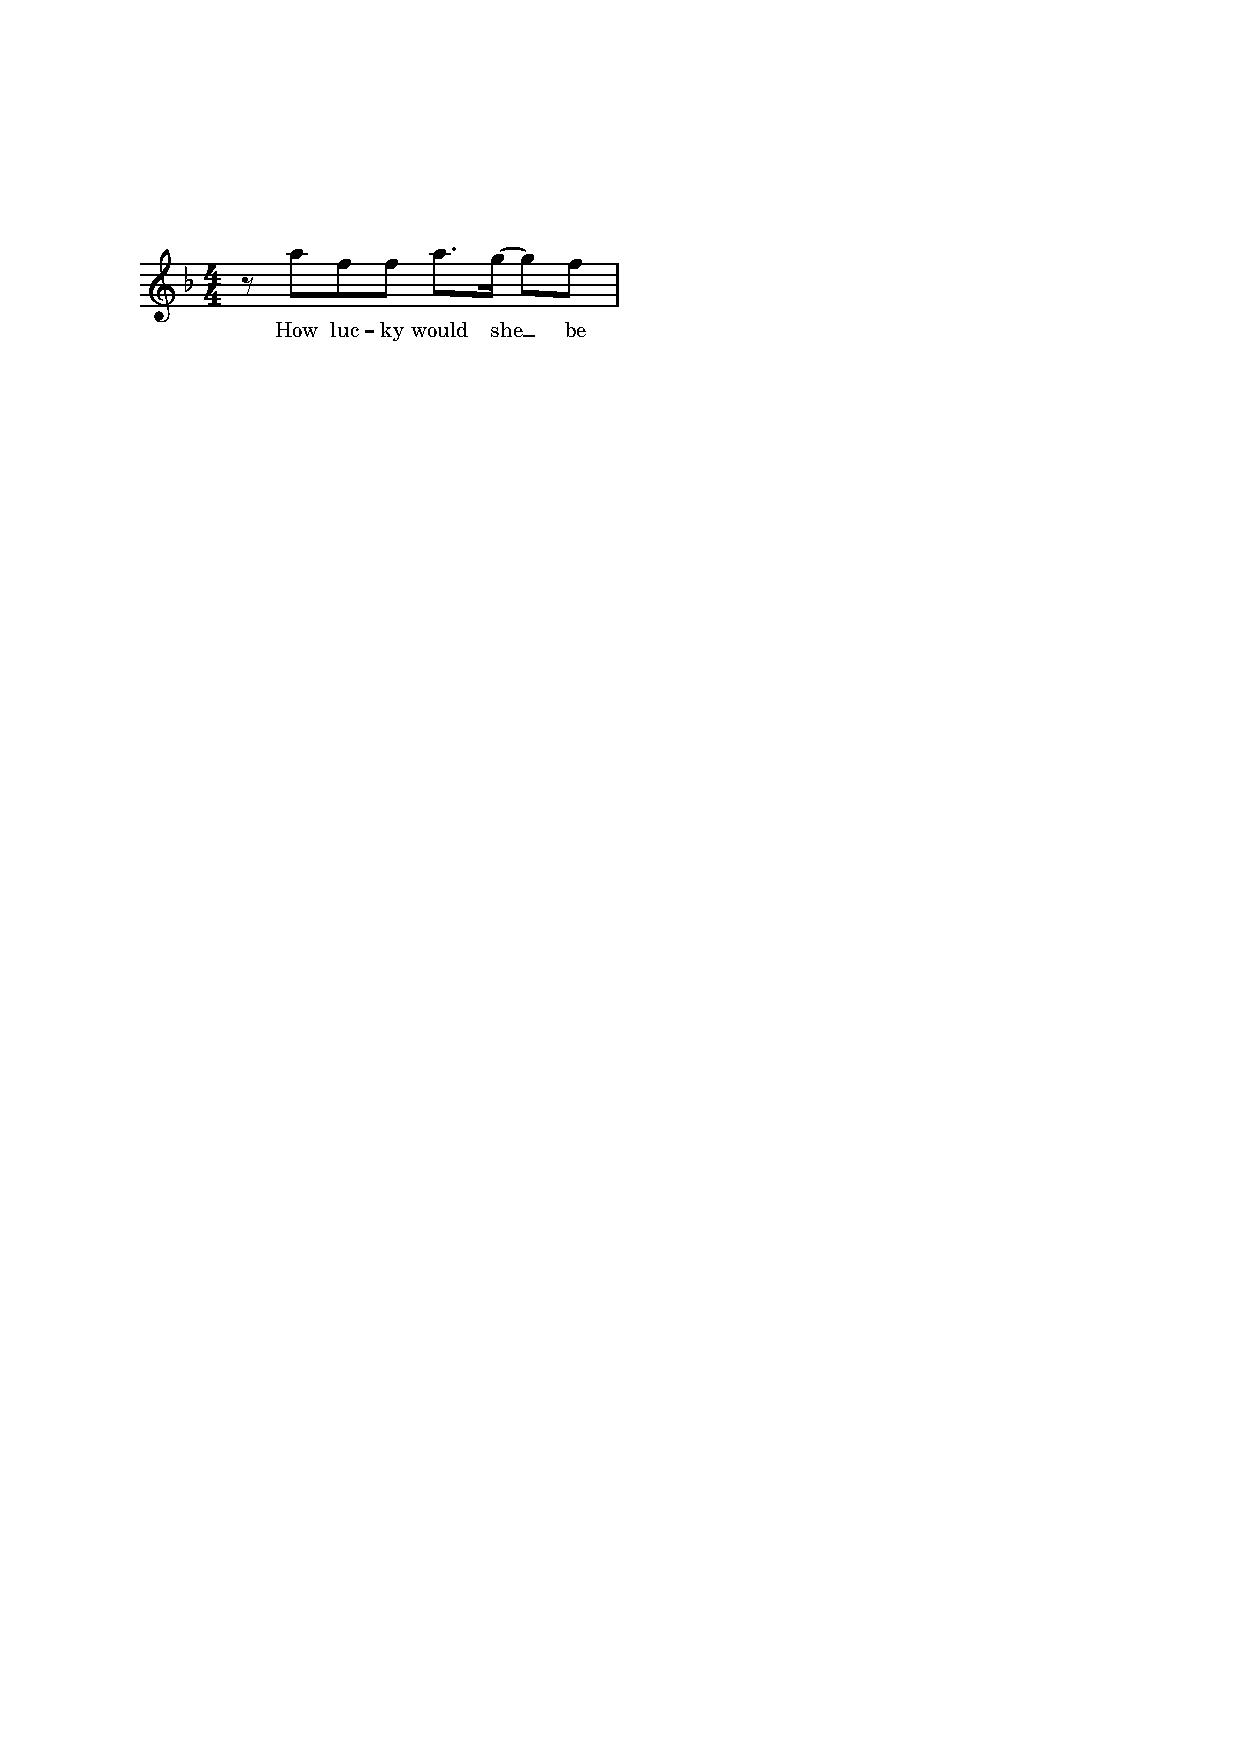
\includegraphics[width=0.44\textwidth,clip=true]{figure/ast/analysis_cases/exp_baseline_en_2.pdf}
}\\
\subfloat[\modelname]{
    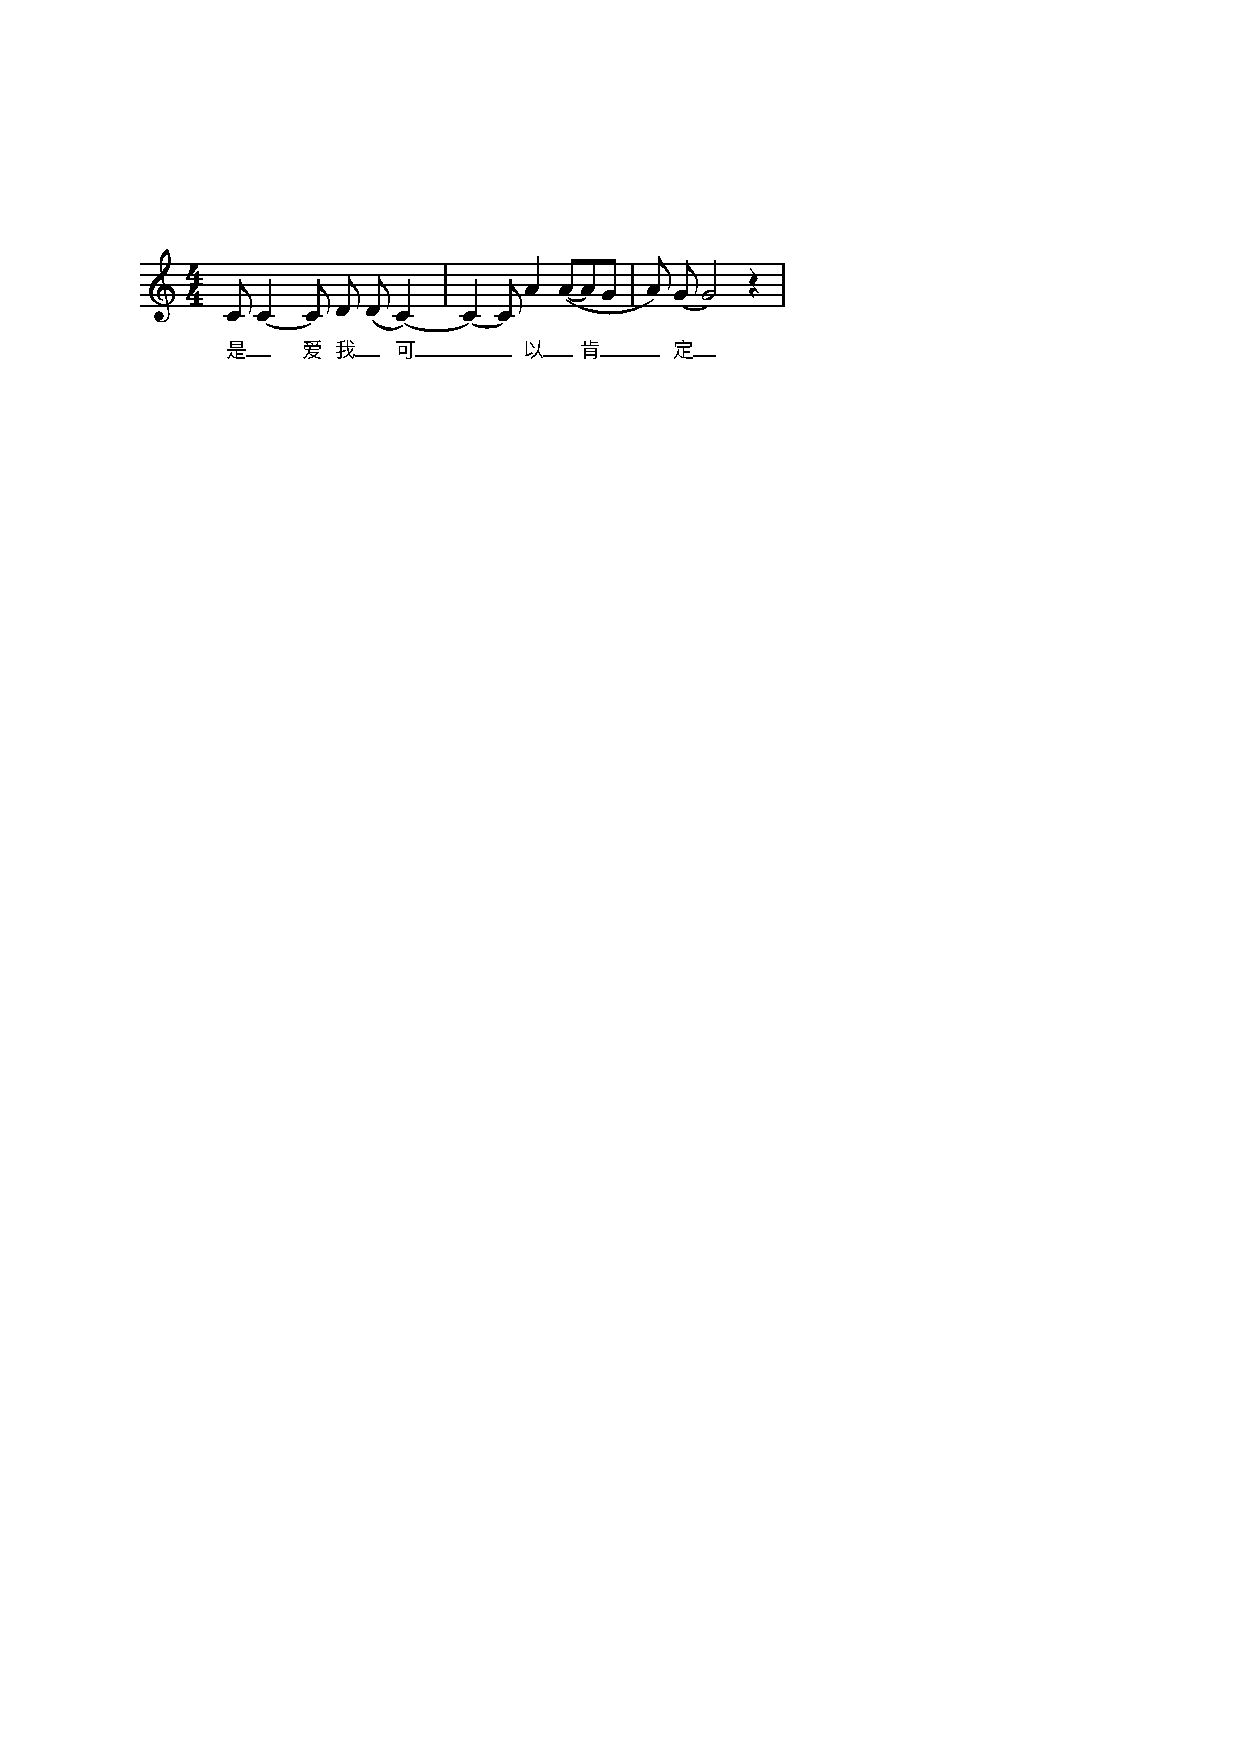
\includegraphics[width=0.55\textwidth,clip=true]{figure/ast/analysis_cases/exp_LTAG_zh_1.pdf}
    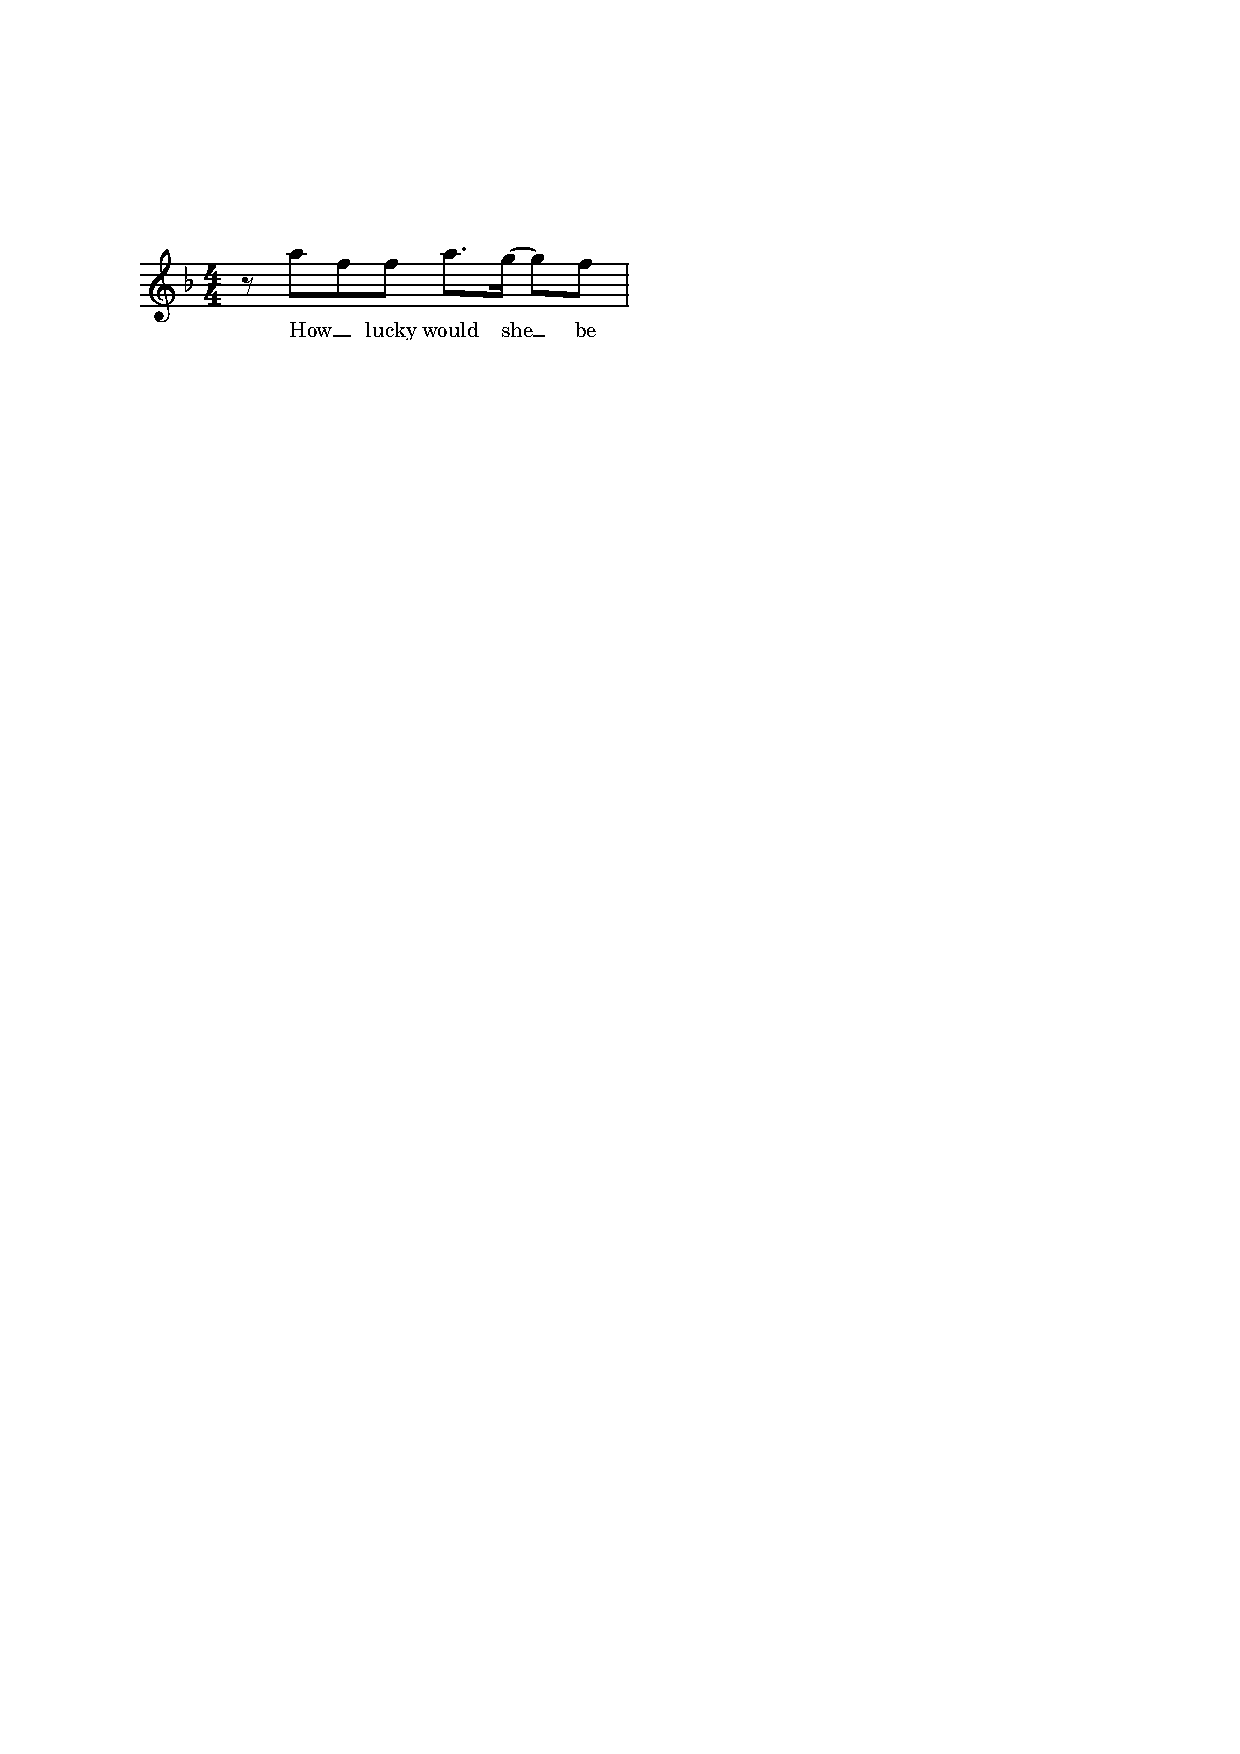
\includegraphics[width=0.44\textwidth,clip=true]{figure/ast/analysis_cases/exp_LTAG_en_2.pdf}
}\\
\caption{Example scores of the source, reference and the translation for ``Is love I can be sure of'' in 《\textit{Will You Love Me Tomorrow}》 and ``她会有多幸运'' in 《\textit{小幸运}》 from three systems.}
\label{fig:score_analysis}
\end{figure}
\section{本章小结}
本章主要针对自动歌曲翻译任务提出了一个完整的。本章提出的,。本章细致阐述了,介绍了本章提出的数据收集方法、实验中使用的数据集情况、。最后,通过对比实验和翻译结果的歌谱展示说明了xxxx取得了更好的文本语义翻译表现和更为合理、更有表现力的歌词-旋律对齐,从而获得了整体上更好的歌曲翻译表现。

\chapter{基于扩散模型的歌声合成}
\section{歌声合成数据集}
PopCS~
\section{歌声合成数据的收集和预处理}
\section{歌声合成的参数前端}
\section{扩散模型}
\subsection{正向扩散过程}
\subsection{反向去噪过程}
\subsection{训练和采样生成}
\section{浅扩散机制}
\subsection{浅扩散机制的原理}
\subsection{浅扩散点的选取}
\section{歌声合成的评价指标}
质量MOS,速度RTF
\section{实验结果与分析}
\section{本章小结}

% \chapter{歌曲到歌声翻译系统}
\section{歌曲翻译结果后处理}

\chapter{总结和展望}
\section{总结}
机器翻译一直以来都是自然语言处理领域针对不同语言文字的一项重要技术。自动歌曲翻译是神经机器翻译在这一基础上针对非常规语体的拓展性研究,这一任务旨在快速地、自动地、高质量地将歌曲的歌词文本翻译到另外一种语言中,同时要求翻译后歌词文本搭配相应旋律依然能以歌曲的形式呈现出来,即翻译后歌词仍能以某种方式来进行艺术性的演唱并传达原意。歌声合成使得直观地呈现歌曲翻译结果成为可能。同时,由于歌声合成可以承接歌曲翻译的输出而连接成为完整的级联式歌曲到歌声的翻译系统,这为歌曲翻译的实际应用打下了坚实的基础。自动歌曲翻译搭配良好的歌声合成效果进行翻唱自动合成,那么听众无需学习多国语言、乐理知识或具备演唱能力就能欣赏来自不同语言不同文化的经典歌曲的母语翻唱版本。
因此,本文提出构建能进行歌词翻译并给出翻译后歌词的合理唱法的翻译模型和高质量的翻唱歌声合成模型以针对歌曲达到自动化地翻译翻唱目的。
本文的主要工作总结如下:

(1)提出了一个能翻译歌词并给出合理的翻译后歌词与原旋律的对齐方式的共同翻译模型。本文提出的歌词和歌词-旋律对齐共同翻译模型是在自回归的基于Transformer的编码器-解码器翻译框架下的改进,模型使用了音符表示池化嵌入层来利用歌词和对齐的输入信息对旋律进行编码。模型使用的轻量的对齐解码器使用了自适应的分组算法来单调地预测歌词和旋律的对齐情况。在本文标注的歌曲翻译数据集上进行的一系列实验和翻译结果的歌谱分析说明了本文提出的歌词和翻译后歌词与原旋律的对齐方式的共同翻译模型取得了更好的文本语义翻译表现和更为合理、更有表现力的歌词-旋律对齐,从而获得了整体上更好的歌曲翻译表现,模型有能力为翻唱提供了优质的歌词和歌谱参照。

(2)搭建了基于扩散模型和对抗训练的翻唱歌声合成声学模型。

同时,两个模型可以进行衔接以形成级联式的自动歌曲翻译翻唱系统,有很强的工业应用价值。
\section{挑战与未来展望}
本文针对自动歌曲翻译和歌声合成这两项任务分别提出了新的模型方法,尽管两个模型在实验中相比于其他现有算法都表现出了很有竞争力的效果,但是仍存在一些不足之处,有进一步优化的空间。主要有以下几点:

本文提出的自动歌曲翻译模型的结果评价在翻译和歌词-旋律对齐质量上都比较依赖人工评测。贵,评测量小
本文在自动歌曲翻译任务中提出的数据收集流程对于收集成千上万句平行语料来说比较合适,对于收集更大量级的数据来说仍比其他这样量级的数据收集流程繁琐很多,且所需技能也需要较长时间的专业训练,更好的自动歌曲翻译数据标注流程亟待探索优化。

本文提出的基于扩散模型的翻唱合成方法虽然合成效果好,训练稳定,但是由于扩散模型迭代进行的去噪过程,为了保证合成效果,去噪模型需要迭代运行数百次,其推理速度和一般的语音合成模型相比有较大的劣势,对于实际落地应用是一个很大的效率问题。之后的研究可以聚焦于扩散模型本身的运行机制或针对这样的合成场景探索在保持合成质量的情况下缩短扩散和逆向过程,或构建更加轻量级、运行更快的去噪模块。

本文提出的两个模型搭建出的级联式系统本身存在误差累积的问题。在自动语音识别、歌曲翻译和歌声合成分别已有相应研究的情况下,探索端到端的歌曲到歌曲翻译模型已成为可能。
